\documentclass[11pt,a4paper]{article}
%DIF LATEXDIFF DIFFERENCE FILE
%DIF DEL C:\Users\ignac\OneDrive\Documentos\GitHub\COTEC-survey-experiment\tmp\paper_A_redline\old.tex   Sun Oct 25 08:29:55 2026
%DIF ADD C:\Users\ignac\OneDrive\Documentos\GitHub\COTEC-survey-experiment\tmp\paper_A_redline\new.tex   Sun Oct 25 08:29:55 2026
\usepackage[utf8]{inputenc}
\usepackage[T1]{fontenc}
\usepackage[english]{babel}
\usepackage{lmodern,microtype,amsmath,amssymb,booktabs,array,graphicx,xcolor,geometry,setspace,float,longtable}
\usepackage{tikz}
\usepackage[section]{placeins}
\usepackage{etoolbox}
\pretocmd{\subsection}{\FloatBarrier}{}{}
\usetikzlibrary{arrows.meta,positioning}
\usepackage[font=small,labelfont=bf]{caption}
\usepackage[authoryear,round]{natbib}
\usepackage[hidelinks]{hyperref}
\geometry{margin=25mm}
\setstretch{1.12}
\setlength{\parskip}{0.35em}
\setlength{\parindent}{1.2em}
\setlength{\emergencystretch}{2em}
\makeatletter
\setlength{\@fptop}{0pt}
\setlength{\@fpsep}{18pt}
\setlength{\@fpbot}{0pt plus 1fil}
\makeatother
\definecolor{reused}{HTML}{000000}
\definecolor{revised}{HTML}{000000}
\definecolor{added}{HTML}{000000}
\newcommand{\old}[1]{{\color{reused}#1}}
\newcommand{\rev}[1]{{\color{revised}#1}}
\newcommand{\new}[1]{{\color{added}#1}}
\newenvironment{addition}{\begingroup\color{added}}{\endgroup}
\newcommand{\pp}{percentage points}
\newcommand{\figroot}{../../3. Output/paper_A/figures/}
\newenvironment{revision}{\begingroup\color{revised}}{\endgroup}
\newcommand{\authors}{\old{Ignacio Garijo-Campos} \and \old{Antonio Alfonso} \and \old{Pablo Bra\~nas-Garza} \and \old{Diego Jorrat} \and \old{Angel Sanchez}}
\newcommand{\plot}[4]{\begin{figure}[!htbp]\centering\begingroup\color{#1}\setlength{\fboxsep}{2pt}\fbox{\includegraphics[width=.94\linewidth]{\figroot#2.png}}\caption{\textcolor{#1}{#3}}\label{#4}\endgroup\end{figure}}
\newcommand{\tabnote}[1]{\par\smallskip{\footnotesize\noindent\textit{Notes:} #1\par}}
\newcommand{\inputtab}[4]{\begin{table}[!htbp]\centering\begingroup\color{#1}\caption{\textcolor{#1}{#3}}\label{#4}\small\input{tables/#2.tex}\endgroup\end{table}}
\date{}
\renewcommand{\floatpagefraction}{0.8}
\renewcommand{\topfraction}{0.9}
\renewcommand{\textfraction}{0.07}
\makeatletter\newcommand{\sectionfloatbarrier}{\ifx\@deferlist\@empty\else\clearpage\fi}\makeatother


\title{“Why Me?”: Understanding Teachers’ Grade-Retention Decisions through a Survey Experiment}
\author{\authors}
%DIF PREAMBLE EXTENSION ADDED BY LATEXDIFF
%DIF UNDERLINE PREAMBLE %DIF PREAMBLE
\RequirePackage[normalem]{ulem} %DIF PREAMBLE
\RequirePackage{color}\definecolor{RED}{rgb}{1,0,0}\definecolor{BLUE}{rgb}{0,0,1} %DIF PREAMBLE
\providecommand{\DIFaddtex}[1]{{\protect\color{blue}\uwave{#1}}} %DIF PREAMBLE
\providecommand{\DIFdeltex}[1]{{\protect\color{red}\sout{#1}}} %DIF PREAMBLE
%DIF SAFE PREAMBLE %DIF PREAMBLE
\providecommand{\DIFaddbegin}{} %DIF PREAMBLE
\providecommand{\DIFaddend}{} %DIF PREAMBLE
\providecommand{\DIFdelbegin}{} %DIF PREAMBLE
\providecommand{\DIFdelend}{} %DIF PREAMBLE
\providecommand{\DIFmodbegin}{} %DIF PREAMBLE
\providecommand{\DIFmodend}{} %DIF PREAMBLE
%DIF FLOATSAFE PREAMBLE %DIF PREAMBLE
\providecommand{\DIFaddFL}[1]{\DIFadd{#1}} %DIF PREAMBLE
\providecommand{\DIFdelFL}[1]{\DIFdel{#1}} %DIF PREAMBLE
\providecommand{\DIFaddbeginFL}{} %DIF PREAMBLE
\providecommand{\DIFaddendFL}{} %DIF PREAMBLE
\providecommand{\DIFdelbeginFL}{} %DIF PREAMBLE
\providecommand{\DIFdelendFL}{} %DIF PREAMBLE
%DIF HYPERREF PREAMBLE %DIF PREAMBLE
\providecommand{\DIFadd}[1]{\texorpdfstring{\DIFaddtex{#1}}{#1}} %DIF PREAMBLE
\providecommand{\DIFdel}[1]{\texorpdfstring{\DIFdeltex{#1}}{}} %DIF PREAMBLE
%DIF AMSMATHULEM PREAMBLE %DIF PREAMBLE
\makeatletter %DIF PREAMBLE
\let\sout@orig\sout %DIF PREAMBLE
\renewcommand{\sout}[1]{\ifmmode\text{\sout@orig{\ensuremath{#1}}}\else\sout@orig{#1}\fi} %DIF PREAMBLE
\makeatother %DIF PREAMBLE
%DIF COLORLISTINGS PREAMBLE %DIF PREAMBLE
\RequirePackage{listings} %DIF PREAMBLE
\RequirePackage{color} %DIF PREAMBLE
\lstdefinelanguage{DIFcode}{ %DIF PREAMBLE
%DIF DIFCODE_UNDERLINE %DIF PREAMBLE
  moredelim=[il][\color{red}\sout]{\%DIF\ <\ }, %DIF PREAMBLE
  moredelim=[il][\color{blue}\uwave]{\%DIF\ >\ } %DIF PREAMBLE
} %DIF PREAMBLE
\lstdefinestyle{DIFverbatimstyle}{ %DIF PREAMBLE
	language=DIFcode, %DIF PREAMBLE
	basicstyle=\ttfamily, %DIF PREAMBLE
	columns=fullflexible, %DIF PREAMBLE
	keepspaces=true %DIF PREAMBLE
} %DIF PREAMBLE
\lstnewenvironment{DIFverbatim}[1][]{\lstset{style=DIFverbatimstyle}}{} %DIF PREAMBLE
\lstnewenvironment{DIFverbatim*}[1][]{\lstset{style=DIFverbatimstyle,showspaces=true}}{} %DIF PREAMBLE
\lstset{extendedchars=\true,inputencoding=utf8}

%DIF END PREAMBLE EXTENSION ADDED BY LATEXDIFF


% Cumulative review styling. Complex deleted exhibits remain intact and red.
\sloppy
\definecolor{deletedreview}{HTML}{B3261E}
\definecolor{addedreview}{HTML}{1756A9}
\renewcommand{\DIFadd}[1]{{\color{addedreview}#1}}
\renewcommand{\DIFdel}[1]{{\color{deletedreview}\sout{#1}}}
\renewcommand{\DIFaddFL}[1]{{\color{addedreview}#1}}
\renewcommand{\DIFdelFL}[1]{{\color{deletedreview}\sout{#1}}}

\begin{document}
\maketitle

\begin{center}\fbox{\begin{minipage}{.94\linewidth}\footnotesize
\textbf{Cumulative review copy.} Compared with the author's version before the coauthor revisions (09f9cd4). Unchanged text is black; \textcolor{addedreview}{additions are blue}; \textcolor{deletedreview}{\sout{deleted text is struck out in red}}. Deleted or superseded exhibits remain visible in red and are explicitly labelled; they are not current results. Moved passages may appear as a deletion at their original location and an addition at their new location.
\end{minipage}}\end{center}


\begin{abstract}
Grade-repetition recommendations translate several kinds of evidence into a binary educational judgment. On the one hand, this decision depends on students' characteristics and educational performance. On the other hand, teachers differ in their level of severity, their opinion on which requirements students should meet for progression, and their cost-benefit assessment of repetition for students' future. We examine this distinction using \DIFdelbegin \DIFdel{22,124 recorded }\DIFdelend \DIFaddbegin \DIFadd{20,467 reconstructed }\DIFaddend recommendations from 2,\DIFdelbegin \DIFdel{705 }\DIFdelend \DIFaddbegin \DIFadd{604 }\DIFaddend teachers in a regional survey experiment in Spain. Within-teacher comparisons show that failed subjects and low basic competences dominate recommendations, with additional contributions from attendance and discipline. \DIFdelbegin \DIFdel{Student complex }\DIFdelend \DIFaddbegin \DIFadd{Complex }\DIFaddend social background reduces recommendations of repetition slightly, while \DIFdelbegin \DIFdel{gender has no significant effect}\DIFdelend \DIFaddbegin \DIFadd{the average gender coefficient is small and statistically indistinguishable from zero}\DIFaddend . Disagreement is greatest when several failed subjects coexist with adequate competences: two teachers evaluating the same recorded profile disagree in 49.1 percent of pairs. We summarize teachers' relative recommendations through a \DIFdelbegin \DIFdel{card-adjusted }\DIFdelend \DIFaddbegin \DIFadd{profile-adjusted }\DIFaddend measure of harshness. Professional characteristics and reported beliefs nevertheless explain little of its variation. A multilevel decomposition assigns \DIFdelbegin \DIFdel{48.63 }\DIFdelend \DIFaddbegin \DIFadd{47.93 }\DIFaddend percent of model-implied decision variation to student attributes and their pairwise interactions, \DIFdelbegin \DIFdel{12.70 }\DIFdelend \DIFaddbegin \DIFadd{12.78 }\DIFaddend percent to observed harshness and \DIFdelbegin \DIFdel{17.10 }\DIFdelend \DIFaddbegin \DIFadd{18.80 }\DIFaddend percent to differences in teachers' attribute sensitivities. Professional characteristics and beliefs together account for less than one percent. The findings distinguish common criteria, disagreement on comparable cases and differences in how teachers apply those criteria.
\end{abstract}
\noindent\textbf{Keywords:} grade repetition; teacher judgment; vignette experiment; harshness; disagreement; variance decomposition.

\section{Introduction}
\DIFdelbegin \DIFdel{Grade-repetition recommendations translate several kinds of evidence into a binary educational judgment. On the one hand, this decision depends on students' characteristics and educational performance. Failed subjects may indicate that a student has not met the requirements for progression. Basic competences provide a partly different signal of what the student can do. Attendance, classroom behavior, and background can further shape how a teacher interprets the difficulty. On the other hand, teachers differ in their level of severity (harshness), their opinion on which requirements students should meet for progression, and their cost-benefit assessment of repetition for students' future}\DIFdelend \DIFaddbegin \DIFadd{Grade retention changes a student's educational trajectory and the peer group in which schooling continues. Its consequences are not uniform: reviews document variation across settings, research designs and comparison groups \mbox{%DIFAUXCMD
\citep{allen,goos,valbuena}}\hskip0pt%DIFAUXCMD
. Social relationships may also be affected. In Spain, a matching-based study associates retention with fewer friendship nominations and greater involvement in hostile peer networks \mbox{%DIFAUXCMD
\citep{branasjorrat}}\hskip0pt%DIFAUXCMD
. These academic and social stakes make it important to understand not only what repetition accomplishes, but how teachers decide whom to recommend for it}\DIFaddend .

\DIFdelbegin \DIFdel{The distinction matters because observed repetition rates combine the situations students face with the judgments applied to those situations}\DIFdelend \DIFaddbegin \DIFadd{Understanding these recommendations requires separating student circumstances from teacher judgment}\DIFaddend . Teachers working with different students can have different repetition rates even if they use the same criteria. Conversely, teachers evaluating comparable students may reach different conclusions. Standardized student profiles allow us to separate these questions more directly than comparisons of `real-world' classroom repetition rates. One reason is that school selection tends to sort similar students into the same schools, meaning that teachers are typically exposed to only a limited range of student profiles rather than to students spanning the full distribution of characteristics. Our experimental design overcomes this limitation by exposing teachers to hypothetical students with systematically varying characteristics.

\DIFdelbegin \DIFdel{The }\DIFdelend \DIFaddbegin \DIFadd{Because the }\DIFaddend educational case for repetition is \DIFdelbegin \DIFdel{itself contingent. Reviews of its consequences document substantial variation across research designs and settings \mbox{%DIFAUXCMD
\citep{allen,goos}}\hskip0pt%DIFAUXCMD
. Evidence that a student faces academic difficulties therefore does }\DIFdelend \DIFaddbegin \DIFadd{contingent, academic difficulties do }\DIFaddend not uniquely determine whether \DIFdelbegin \DIFdel{repetition }\DIFdelend \DIFaddbegin \DIFadd{another year in the same grade }\DIFaddend is an appropriate response. Our \DIFdelbegin \DIFdel{conceptual }\DIFdelend framework distinguishes teachers' assessment of difficulties if the student progresses from their assessment of the gains and costs of making the student repeat. \DIFdelbegin \DIFdel{This distinction organizes the interpretation of academic signals, behavioral information and social circumstances without assuming that one recommendation is universally correct.

}%DIFDELCMD < 

%DIFDELCMD < %%%
\DIFdel{We study 2,705 teachers evaluating profiles with six attributes. The analysis addresses three connected questions. First, which attributes change recommendations within teachers? Second, how much do teachers differ when the information is comparable, and which cases divide them? Third, how do student information, teacher characteristics and observed patterns of teacher judgment contribute to variation in recommendations? A measure of }\textit{\DIFdel{harshness}}%DIFAUXCMD
\DIFdel{, defined as the average deviation from other teachers' recommendations on the same cards, connects the second and third }\DIFdelend \DIFaddbegin \DIFadd{Studies of recommendations and studies of the consequences of actual retention therefore address complementary }\DIFaddend questions.

\DIFdelbegin \DIFdel{Studying these questions together helps distinguish disagreement on individual cases from broader patterns in teachers' recommendations. Disagreement over one student profile need not imply that the same teachers also differ across other profiles. If some teachers repeatedly recommend retention more often than their peers on comparable cases, however, there is a pattern to explain---even if their observed characteristics provide little help in predicting it.

}%DIFDELCMD < 

%DIFDELCMD < %%%
\DIFdel{The results distinguish all three levels. Firstly, failed subjects and low competences have the largest within-teacher coefficients, 54.6 and 27.1 percentage points, and reinforce one another in an interaction specification. Attendance and discipline also matter (6.4 and 4.6 p.p. respectively). Complex social background moderates repetition recommendations (-1.9 p.p.), and gender has a small and not significant average coefficient. These last two findings contrast with the higher repetition incidence among boys and disadvantaged students documented in population data \mbox{%DIFAUXCMD
\citep{oecd}}\hskip0pt%DIFAUXCMD
, which suggests that teachers do not penalize these characteristics. 

}%DIFDELCMD < 

%DIFDELCMD < %%%
\DIFdel{Secondly, harshness varies substantially across teachers. Disagreement is especially pronounced for several failed subjects combined with adequate competences. Thirdly, demographic and professional information, together with reported beliefs, explains less than five percent of observed harshness variation. The decision-level decomposition shows that student information contributes most, while general harshness and differences in the weight teachers give individual attributes each account for substantial additional components. The contribution is thus to connect common criteria, disagreement on comparable cases and differences in how those criteria are applied.

}%DIFDELCMD < 

%DIFDELCMD < %%%
\section*{\DIFdel{Related literature}}
%DIFAUXCMD

\DIFdel{The first literature concerns the consequences of retaining students. \mbox{%DIFAUXCMD
\citet{allen} }\hskip0pt%DIFAUXCMD
find less negative estimated achievement effects in stronger research designs. \mbox{%DIFAUXCMD
\citet{goos} }\hskip0pt%DIFAUXCMD
report an average effect near zero alongside heterogeneity across contexts, comparisons and outcomes. These findings motivate attention to how teachers make recommendations; they do not supply a universal decision rule for every student profile. Studies of recommendations and studies of the consequences of actual retention address complementary questions}\DIFdelend \DIFaddbegin \DIFadd{Teachers' judgments can incorporate information beyond demonstrated academic performance. Comparing teacher-assigned and blindly assigned scores in Brazil, \mbox{%DIFAUXCMD
\citet{ferman} }\hskip0pt%DIFAUXCMD
find that classroom behavior enters grading and promotion decisions. In a British experiment, \mbox{%DIFAUXCMD
\citet{doyle} }\hskip0pt%DIFAUXCMD
find that an identical piece of written work receives less favorable evaluations when attributed to a student of lower socioeconomic status. These studies motivate separating academic signals, conduct and social circumstances, while recognizing that grading a piece of work and recommending grade retention are different judgments}\DIFaddend .

Research on \DIFdelbegin \DIFdel{teachers' }\DIFdelend \DIFaddbegin \DIFadd{retention }\DIFaddend beliefs provides a \DIFdelbegin \DIFdel{second }\DIFdelend \DIFaddbegin \DIFadd{complementary }\DIFaddend foundation. Tomchin and Impara \citeyearpar{tomchin} examine the reasoning underlying retention judgments, and \citet{bonvin} connects attitudes and judgments to retention decisions. \DIFdelbegin \DIFdel{This work motivates our distinction between diagnosing a difficulty and considering repetition an appropriate response. }\DIFdelend Beliefs are not a single construct: \DIFdelbegin \DIFdel{reports of }\DIFdelend empathy, views about the role of effort and assessments of educational resources capture different considerations \citep{pajares}. We use these measures to characterize observed harshness and to distinguish measured teacher information from patterns revealed by \DIFdelbegin \DIFdel{their }\DIFdelend decisions.

Klapproth and Beyte \citeyearpar{klapproth} provide a close experimental antecedent. Their 146 participants, including 108 teachers in training and 38 practicing teachers, evaluate profiles varying in grades, subject of failure and gender. They also complete a 16-item retention-attitude questionnaire. Both studies use vignettes to connect student information and teacher characteristics to recommendations. Our larger sample of practicing teachers permits a more detailed study of disagreement and variation in teacher judgment. The profile design adds attendance, discipline and social context, and distinguishes failed subjects from basic competences. It therefore addresses conflicts between formal performance and competence rather than differences between subject domains. Our broader professional information and beliefs extending beyond retention also answer a different measurement question; their questionnaire measures retention-specific attitudes more intensively.

Multidimensional vignette designs allow researchers to study how several characteristics jointly enter a judgment \citep{conjoint}. Here, variation within teachers identifies changes in recommendations, while repeated profiles locate disagreement across teachers. We complement these comparisons with a model-based decomposition that distinguishes student information, observed teacher characteristics, overall harshness and teacher-specific responses to attributes.

\DIFaddbegin \DIFadd{We study 2,604 teachers evaluating profiles with six attributes. Four questions organize the contribution: which attributes change recommendations within teachers; how academic and behavioral signals combine; where teachers disagree on comparable cases; and how measured teacher information and observed response patterns contribute to decision variation. The first two questions form the within-teacher results, the third motivates the between-teacher analysis, and the fourth connects teacher characteristics to the decomposition. Harshness, defined as the average departure from other teachers' recommendations on the same six-attribute profiles, links these analyses.

}

\DIFadd{Studying these questions together helps distinguish disagreement on individual cases from broader patterns in teachers' recommendations. Disagreement over one student profile need not imply that the same teachers also differ across other profiles. If some teachers repeatedly recommend retention more often than their peers on comparable cases, however, there is a pattern to explain---even if their observed characteristics provide little help in predicting it.

}

\DIFadd{The results distinguish common criteria from their application. Failed subjects and low competences have the largest within-teacher coefficients, 54.7 and 27.1 percentage points, and reinforce one another. Attendance and discipline also matter (6.7 and 4.8 points). Complex social background moderates repetition recommendations ($-1.8$ points), whereas the average gender coefficient is small and statistically indistinguishable from zero. The contrast with higher repetition incidence among boys and disadvantaged students in population data \mbox{%DIFAUXCMD
\citep{oecd} }\hskip0pt%DIFAUXCMD
is compatible with disparities arising partly before the final promotion judgment, rather than from an additional penalty attached directly to these characteristics in otherwise comparable cases.

}

\DIFadd{Harshness varies substantially across teachers, and disagreement is particularly pronounced for several failed subjects combined with adequate competences. Demographic and professional information and reported beliefs explain less than five percent of observed harshness variation. The decision-level decomposition assigns the largest share to student information, with substantial additional components associated with overall harshness and different responses to attributes. The contribution is to connect common criteria, disagreement on comparable cases and differences in how those criteria are applied.

}

\DIFaddend \section{Study design and measurement}
\subsection{Participants and questionnaire}
The survey was collected between 14 March and 29 April 2025 among primary and secondary teachers in one Spanish region. The study plan specifies recruitment through the regional education authority and schools forwarding an online questionnaire. Participation was voluntary. After setting aside 905 entries with minimal initial engagement, 4,037 records form the participation-flow denominator\DIFdelbegin \DIFdel{. Of these, }\DIFdelend \DIFaddbegin \DIFadd{; }\DIFaddend 3,103 contain \DIFdelbegin \DIFdel{a response to }\DIFdelend at least one card \DIFaddbegin \DIFadd{response}\DIFaddend , including examples. The \DIFaddbegin \DIFadd{favorable-example }\DIFaddend screening rule excludes \DIFdelbegin \DIFdel{389, and nine further recordscontain only responses in fields omitted from the analytical outcome}\DIFdelend \DIFaddbegin \DIFadd{379 records. A further 120 lack a recoverable experimental response}\DIFaddend , leaving 2,\DIFdelbegin \DIFdel{705 teachers with usable }\DIFdelend \DIFaddbegin \DIFadd{604 teacher records with 20,467 }\DIFaddend recommendations. Appendix~\ref{app:sample} documents \DIFdelbegin \DIFdel{participation, card completion, response times }\DIFdelend \DIFaddbegin \DIFadd{this reconstruction, participation }\DIFaddend and comparisons with regional teacher statistics.

The initial questionnaire asks about teachers' demographic and professional circumstances: their age and gender, years of teaching, educational stage, employment situation, school ownership and number of teaching groups. Teachers then consider hypothetical students and choose whether each should progress or repeat. The cards describe 6 binary characteristics gender, and whether the student comes from a complex social background, has failed 3 or more subjects, presents low basic competences, has been absent frequently, and has disciplinary problems. Two examples introduce this task before the eight experimental cards.

The six vignette attributes cover academic standing, school engagement and conduct, and sociodemographic background. Prior research links grade retention to school grades \citep{klapprothschaltz2015retained} and academic skills \citep{davoudzadeh2015readiness}. Separate indicators of failed subjects and basic competences allow us to examine how teachers weigh these signals when they diverge. Teachers report considering attendance in retention decisions \citep{santosmonteiro2024retention}, and longitudinal evidence links teacher-rated externalizing behavior to subsequent retention \citep{mattison2018behavior}. Gender and social background address documented demographic and socioeconomic disparities in retention \citep{gonzalezbetancor2016retention,klapprothschaltz2015retained}. Varying these characteristics alongside academic and behavioral information allows us to examine whether they enter recommendations for otherwise comparable student profiles.

\DIFaddbegin \DIFadd{Teachers were randomly assigned to one of eight predefined sets of eight cards, with randomized presentation order within the set. The 64 set positions represent 56 distinct six-attribute profiles: eight profiles occur in two sets, and eight of the 64 possible combinations are absent. Gender and social background are balanced within each set, but the academic and behavioral composition differs across sets (Appendix~\ref{app:sample}). The survey also assigned policy-information contexts, including a control condition. This article pools recommendations across those contexts; a control-only attribute comparison is reported in the appendix.

}

\DIFaddend The \DIFaddbegin \DIFadd{student-profile decision task was documented in the study's preregistration \mbox{%DIFAUXCMD
\citep{registry}}\hskip0pt%DIFAUXCMD
. We use this registered task to study how student information and differences between teachers structure recommendations. The reconstruction and the covariance comparisons reported here were developed for the present analysis.

}

\DIFadd{The }\DIFaddend final questionnaire asks teachers to assess their influence on students, describe their empathy, and judge the role of effort rather than luck or family circumstances in economic outcomes. It also asks about resources for students who repeat, including agreement that too many resources are devoted to them. These questions capture professional self-perceptions and broader beliefs alongside views directly relevant to repetition. Figure~\ref{fig:timeline} shows when the two questionnaires and the decisions occur.



\begin{figure}[!htbp]\centering
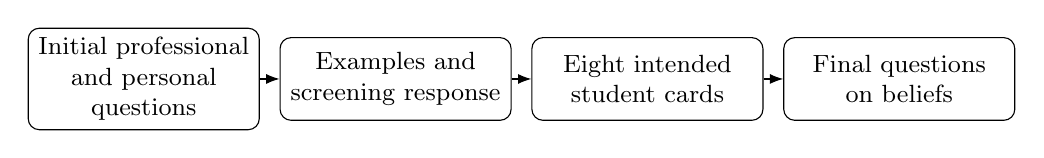
\begin{tikzpicture}[n/.style={draw,rounded corners,align=center,text width=2.7cm,minimum height=1.05cm,font=\small},>=Latex]
\node[n] (a) {Initial professional\\and personal questions};
\node[n,right=0.25cm of a] (b) {Examples and\\screening response};
\node[n,right=0.25cm of b] (c) {Eight intended\\student cards};
\node[n,right=0.25cm of c] (d) {Final questions\\on beliefs};
\draw[->] (a)--(b);\draw[->] (b)--(c);\draw[->] (c)--(d);
\end{tikzpicture}
\caption{Timing of the measurements used here, within one survey encounter. Belief reports follow the recommendations.}\label{fig:timeline}
\end{figure}


Before the task, teachers are shown \DIFdelbegin \DIFdel{two examples. One is an ideal student with no negative characteristics. The other is a student with all characteristics associated with grade repetition . These examples were included to make the task clear and to work as an attention check. We removed teachers that failed the student with none of the characteristics associated with grade repetition.

We decided not to remove teachers that did not fail the student with all before-mentioned characteristics,since some teachers do not believe in grade repetition at all}\DIFdelend \DIFaddbegin \DIFadd{a favorable example and an example combining adverse academic and behavioral characteristics. We exclude records recommending repetition for the favorable example assigned to that respondent. We do not exclude teachers who recommend progression for the adverse example, since they may oppose repetition even in difficult cases. The rule is an outcome-based analytical screen, not independent evidence of inattention; the appendix therefore also reports results without it.

}

\DIFadd{We reconstruct experimental responses from each record's eight-position presentation sequence, keeping only assigned card fields. When an assigned card and that respondent's example share a stored response field, reconstruction B retains that value once, assuming that the recommendation is unchanged between the example and experimental presentation. There are 656 such retained observations. Excluding these shared values provides a sensitivity check; it removes ambiguity but also selectively removes extreme profiles. The main sample retains up to eight observed recommendations per teacher: 2,520 teachers have eight and 84 have one to seven}\DIFaddend .

\section{Decision framework and empirical strategy}
\subsection{Diagnosing difficulty and choosing an educational response}

A recommendation to repeat can reflect both concern about progression and a view about what repetition would accomplish. Let $x_i$ denote student $i$'s profile. Teacher $j$ perceives a probability $q(x_i,z_j,\eta_j^q)$ of consequential difficulty if the student progresses, a gain $g(x_i,z_j,\eta_j^g)$ from repetition rather than progression when that difficulty occurs, and a cost $c(x_i,z_j,\eta_j^c)$ of repetition. A compact decision rule is
\[
Y_{ij}=\mathbf{1}\{q(x_i,z_j,\eta_j^q)g(x_i,z_j,\eta_j^g)>c(x_i,z_j,\eta_j^c)\}.
\]
This representation concentrates benefits in the event of difficulty and measures benefits and costs on a compatible scale.

Here, $z_j$ collects the teacher characteristics and beliefs measured in the survey. The terms $\eta_j^q$, $\eta_j^g$, and $\eta_j^c$ represent unmeasured aspects of the teacher's judgment concerning the risks of progression, the benefits of repetition, and its costs, respectively. For example, teachers with similar observed characteristics may interpret the same failed subjects differently or disagree about whether another year would address the underlying difficulty. These differences may affect both their overall willingness to recommend repetition and the weight they place on particular student attributes. The framework distinguishes these possible sources of disagreement; our data do not identify the three components separately.

The distinction supplies three useful implications. First, teachers can agree that a student faces difficulties but disagree about whether repeating is the appropriate response. Second, a difficult social context can increase concern about progression while also increasing the perceived costs of retention or reducing its expected gains. A negative background coefficient therefore need not indicate less concern about the student. Third, a common average tendency does not exhaust differences of judgment: teachers with similar harshness can disagree about which students should repeat.

Academic performance informs both the diagnosis and the possible benefit of repeating. Attendance and disciplinary problems can inform assessments of readiness, engagement and how another year would work. Gender and social circumstances can affect interpretations of the same information. 



\subsection{Within-teacher responses to student information}
We estimate linear probability models with teacher fixed effects and standard errors clustered by teacher. The fixed effects absorb differences in average recommendation levels\DIFdelbegin \DIFdel{; the attribute coefficients summarize changes across the cards a teacher evaluates}\DIFdelend \DIFaddbegin \DIFadd{, including any constant set or policy-context effect within teacher. Attribute coefficients summarize conditional contrasts across the implemented profiles, rather than averages over independently randomized attributes in the full factorial}\DIFaddend . Teachers with only one usable response contribute to descriptive harshness but not to \DIFdelbegin \DIFdel{identification of these coefficients. The main specification therefore contains 22,006 }\DIFdelend \DIFaddbegin \DIFadd{these coefficients; the main specification contains 20,452 }\DIFaddend decisions from 2,\DIFdelbegin \DIFdel{587 teachers. }\DIFdelend \DIFaddbegin \DIFadd{589 teachers. The fixed effects do not require attribute responses to be identical across policy contexts.

}\DIFaddend 

The additive model includes all six attributes. An interaction model adds failed subjects interacted with competences, absence and discipline, with Holm adjustment across those three interaction tests. The within-teacher analysis asks which student information changes recommendations, while the teacher-level models examine differences in harshness. Student attributes are denoted by $x_i$; $X_1$--$X_3$ below label sets of teacher covariates.

\subsection{Harshness and disagreement between teachers}
We define \textit{harshness} as the teacher's relative propensity to recommend repetition on the cards answered. For each response, the comparison is the repetition rate among other teachers evaluating the same \DIFdelbegin \DIFdel{recorded card}\DIFdelend \DIFaddbegin \DIFadd{six-attribute profile, pooling identifiers with identical attributes}\DIFaddend :
\[
d_{ij}=Y_{ij}-\overline Y_{i,-j},\qquad
H^b_j=\frac{1}{n_j}\sum_{i\in I_j}d_{ij}.
\]
A value of 0.10 means ten percentage points above the references for those cards, on average. The label does not imply that recommending repetition is wrong. Comparing with the \DIFdelbegin \DIFdel{same-card }\DIFdelend \DIFaddbegin \DIFadd{same-profile }\DIFaddend reference accounts for the observed profile mix, while the finite number of responses limits how precisely each teacher can be measured.

We present the distribution of $H^b$ (Figure~\ref{fig:harshness}) and use terciles to describe how attribute coefficients differ across it. Our harshness measure lies between $-1$ and 1, with higher values indicating greater severity relative to peers. A teacher with a score of zero is, on average, as harsh as peers evaluating the same cards. The response-weighted mean is zero by construction; the unweighted mean across teachers need not be zero because teachers contribute different numbers of responses.

Harshness summarizes the direction of a teacher's departures from peers. Same-profile disagreement \DIFdelbegin \DIFdel{instead }\DIFdelend asks whether two distinct teachers evaluating an identical \DIFdelbegin \DIFdel{identifier }\DIFdelend \DIFaddbegin \DIFadd{six-attribute profile }\DIFaddend recommend different outcomes. We calculate this probability within each \DIFdelbegin \DIFdel{identifier }\DIFdelend \DIFaddbegin \DIFadd{profile }\DIFaddend and average it by \DIFdelbegin \DIFdel{observed }\DIFdelend response frequency, including within four categories formed by failed subjects and competences. \DIFdelbegin \DIFdel{The two statistics are complementary: similar average harshness need not imply agreement on individual students}\DIFdelend \DIFaddbegin \DIFadd{Thus repeated profiles under different set identifiers contribute to the same reference. The appendix checks the alternative of retaining identifier-specific references.

}

\DIFadd{These comparisons pool the survey's randomized policy-information contexts. Harshness and same-profile disagreement can therefore reflect context-related responses as well as differences between teachers; they are not estimates of stable teacher traits isolated from the survey encounter}\DIFaddend .

\subsection{Teacher characteristics and sources of decision variation}
Harshness is the dependent variable in the teacher-level models. The professional and demographic set, $X_1$, contains educational stage, experience, gender, age, school ownership, reported permanent public appointment and number of teaching groups. $X_2$ adds perceived teacher impact, empathy and attribution of economic position to effort rather than luck. $X_3$ adds agreement that too many resources are allocated to repeaters, on its original 0--10 scale. The effort item runs from 1 (luck, family circumstances and contacts) to 10 (effort, education and merit).

All three specifications use the same 2,\DIFdelbegin \DIFdel{157 }\DIFdelend \DIFaddbegin \DIFadd{164 }\DIFaddend complete cases. We use HC3 robust standard errors to allow for differences in residual variability across teachers, with an additional adjustment for unusual combinations of teacher characteristics.

\subsection{Decomposing variation in recommendations}
The final analysis asks how much variation in recorded decisions is represented by the information assembled in the paper. We distinguish the student's profile, the teacher's measured characteristics and beliefs, the teacher's overall harshness, and differences in the importance teachers attach to each attribute. These last two components answer different questions: harshness describes whether a teacher recommends repetition more often overall, whereas attribute sensitivities describe which kinds of students elicit a stronger response from that teacher.

We estimate a linear mixed model on the \DIFdelbegin \DIFdel{18,608 }\DIFdelend \DIFaddbegin \DIFadd{17,312 }\DIFaddend decisions of the 2,\DIFdelbegin \DIFdel{157 }\DIFdelend \DIFaddbegin \DIFadd{164 }\DIFaddend complete-case teachers:
\begin{equation}
Y_{ij}=\alpha+f(x_i)+z_j'\gamma+a_j'\delta+\rho H^b_j+
\widetilde{x}_i'b_j+\varepsilon_{ij},
\label{eq:decomposition}
\end{equation}
where $f(x_i)$ contains the six student attributes and all 15 pairwise interactions, $z_j$ contains professional and demographic characteristics, and $a_j$ contains \DIFdelbegin \DIFdel{the }\DIFdelend reported beliefs. The six elements of $b_j$ are teacher-specific deviations from the average attribute coefficients\DIFdelbegin \DIFdel{, modeled jointly with an unrestricted covariance matrix }\DIFdelend \DIFaddbegin \DIFadd{. The primary model estimates a separate variance for each deviation and sets their covariances to zero, so }\DIFaddend $\Sigma$ \DIFdelbegin \DIFdel{. The random-slope predictors }\DIFdelend \DIFaddbegin \DIFadd{is diagonal. Predictors }\DIFaddend $\widetilde{x}_i$ are centered at their means across the \DIFdelbegin \DIFdel{observed }\DIFdelend \DIFaddbegin \DIFadd{complete-case }\DIFaddend decisions. For example, \DIFdelbegin \DIFdel{two }\DIFdelend teachers with the same overall harshness can attach different additional weight to absenteeism\DIFdelbegin \DIFdel{. Its }\DIFdelend \DIFaddbegin \DIFadd{: its }\DIFaddend common coefficient captures the average response\DIFdelbegin \DIFdel{; }\DIFdelend \DIFaddbegin \DIFadd{, while }\DIFaddend its random slope allows that response to differ across teachers. All six attributes receive random slopes\DIFdelbegin \DIFdel{, including those with small average coefficients}\DIFdelend . The model includes neither an additional teacher random intercept nor experimental-assignment indicators.

\DIFaddbegin \DIFadd{The diagonal specification is the stable interior solution among three covariance structures compared on the same data. We retain correlated-pair and unrestricted specifications as sensitivities in Appendix~\ref{app:prediction}. Zero covariances are a working restriction, not a finding that teachers' responses to different attributes are unrelated.

}

\DIFaddend For the allocation, let $\widehat m_{ij}$ be the fitted fixed part of Equation~\ref{eq:decomposition}. We define total model-implied variance as
\begin{equation}
T=\operatorname{Var}(\widehat m_{ij})+
\frac{1}{N}\sum_{ij}\widetilde{x}_i'\widehat\Sigma\widetilde{x}_i+
\widehat\sigma^2.
\label{eq:variance_total}
\end{equation}
The second term measures the joint contribution of attribute sensitivities over the observed profiles\DIFdelbegin \DIFdel{, including their covariances}\DIFdelend \DIFaddbegin \DIFadd{; in the diagonal specification it is the sum of each slope variance multiplied by its centered predictor's mean square}\DIFaddend . The third is remaining decision-level variation. This averages random-slope variance across the observed design rather than treating each slope variance as a separate additive share \citep{nakagawa}.

Student attributes, professional characteristics, beliefs and harshness share information. To divide $\operatorname{Var}(\widehat m)$ without choosing a favorable order of entry, we use a Shapley allocation \citep{groemping}. For each subset of these four blocks, we project the same full-model predictor onto that subset and measure the variance of the projection. A block's contribution is its average increment across all 24 possible orders. Thus we allocate one fitted predictor; we do not repeatedly estimate reduced mixed models. Dividing these four contributions, the joint sensitivity variance and the residual variance by $T$ produces six shares summing to 100 percent. Each decision receives equal weight.

This allocation describes the structure of the observed recommendations. Harshness is calculated from those same recommendations, so its contribution summarizes information extracted from the decisions, rather than information available before a teacher answers. The percentages are neither classification accuracy nor demonstrated prediction for new teachers. Restricted maximum likelihood estimates the variance components. Teacher bootstrap samples rebuild the \DIFdelbegin \DIFdel{same-card }\DIFdelend \DIFaddbegin \DIFadd{same-profile }\DIFaddend references and harshness before refitting the full model and allocation; Appendix~\ref{app:prediction} reports computational details and diagnostics.

\section{Results}
\subsection{Within teachers: how student information changes recommendations}
The within-teacher coefficients in \DIFdelbegin \DIFdel{Table~\ref{tab:attr} }\DIFdelend \DIFaddbegin \DIFadd{Figure~\ref{fig:attributes} }\DIFaddend show a clear hierarchy of information. Three or more failed subjects increase the recommendation probability by about 55 percentage points, and low basic competences by about 27 points. These academic indicators convey different information: failed subjects refer to formal performance, whereas competences describe preparedness more broadly.



\DIFdelbegin 
\begin{table}[!htbp]
\centering\begingroup\color{deletedreview}
\caption*{\textcolor{deletedreview}{\textbf{Deleted / superseded --- baseline Table 1.} Within-teacher responses to student attributes}}
\small
\begin{tabular}{lr}
\toprule
Attribute & Coefficient (SE) \\
\midrule
Three or more failed subjects & \shortstack{54.62$^{***}$\\{\scriptsize (0.71)}} \\
Low basic competences & \shortstack{27.07$^{***}$\\{\scriptsize (0.63)}} \\
Frequent unjustified absence & \shortstack{6.37$^{***}$\\{\scriptsize (0.43)}} \\
Serious disciplinary problems & \shortstack{4.56$^{***}$\\{\scriptsize (0.48)}} \\
Male student & \shortstack{0.26\\{\scriptsize (0.45)}} \\
Complex social background & \shortstack{-1.88$^{***}$\\{\scriptsize (0.44)}} \\
\bottomrule
\end{tabular}
\tabnote{Coefficients in percentage points from additive teacher fixed-effect models; teacher-clustered SE. 22,006 decisions from 2,587 teachers. $^{*}p<.05$, $^{**}p<.01$, $^{***}p<.001$. SE in parentheses.}

\endgroup\end{table}


\DIFdelend \DIFaddbegin 
\begin{figure}[!htbp]
\centering\begingroup\color{addedreview}
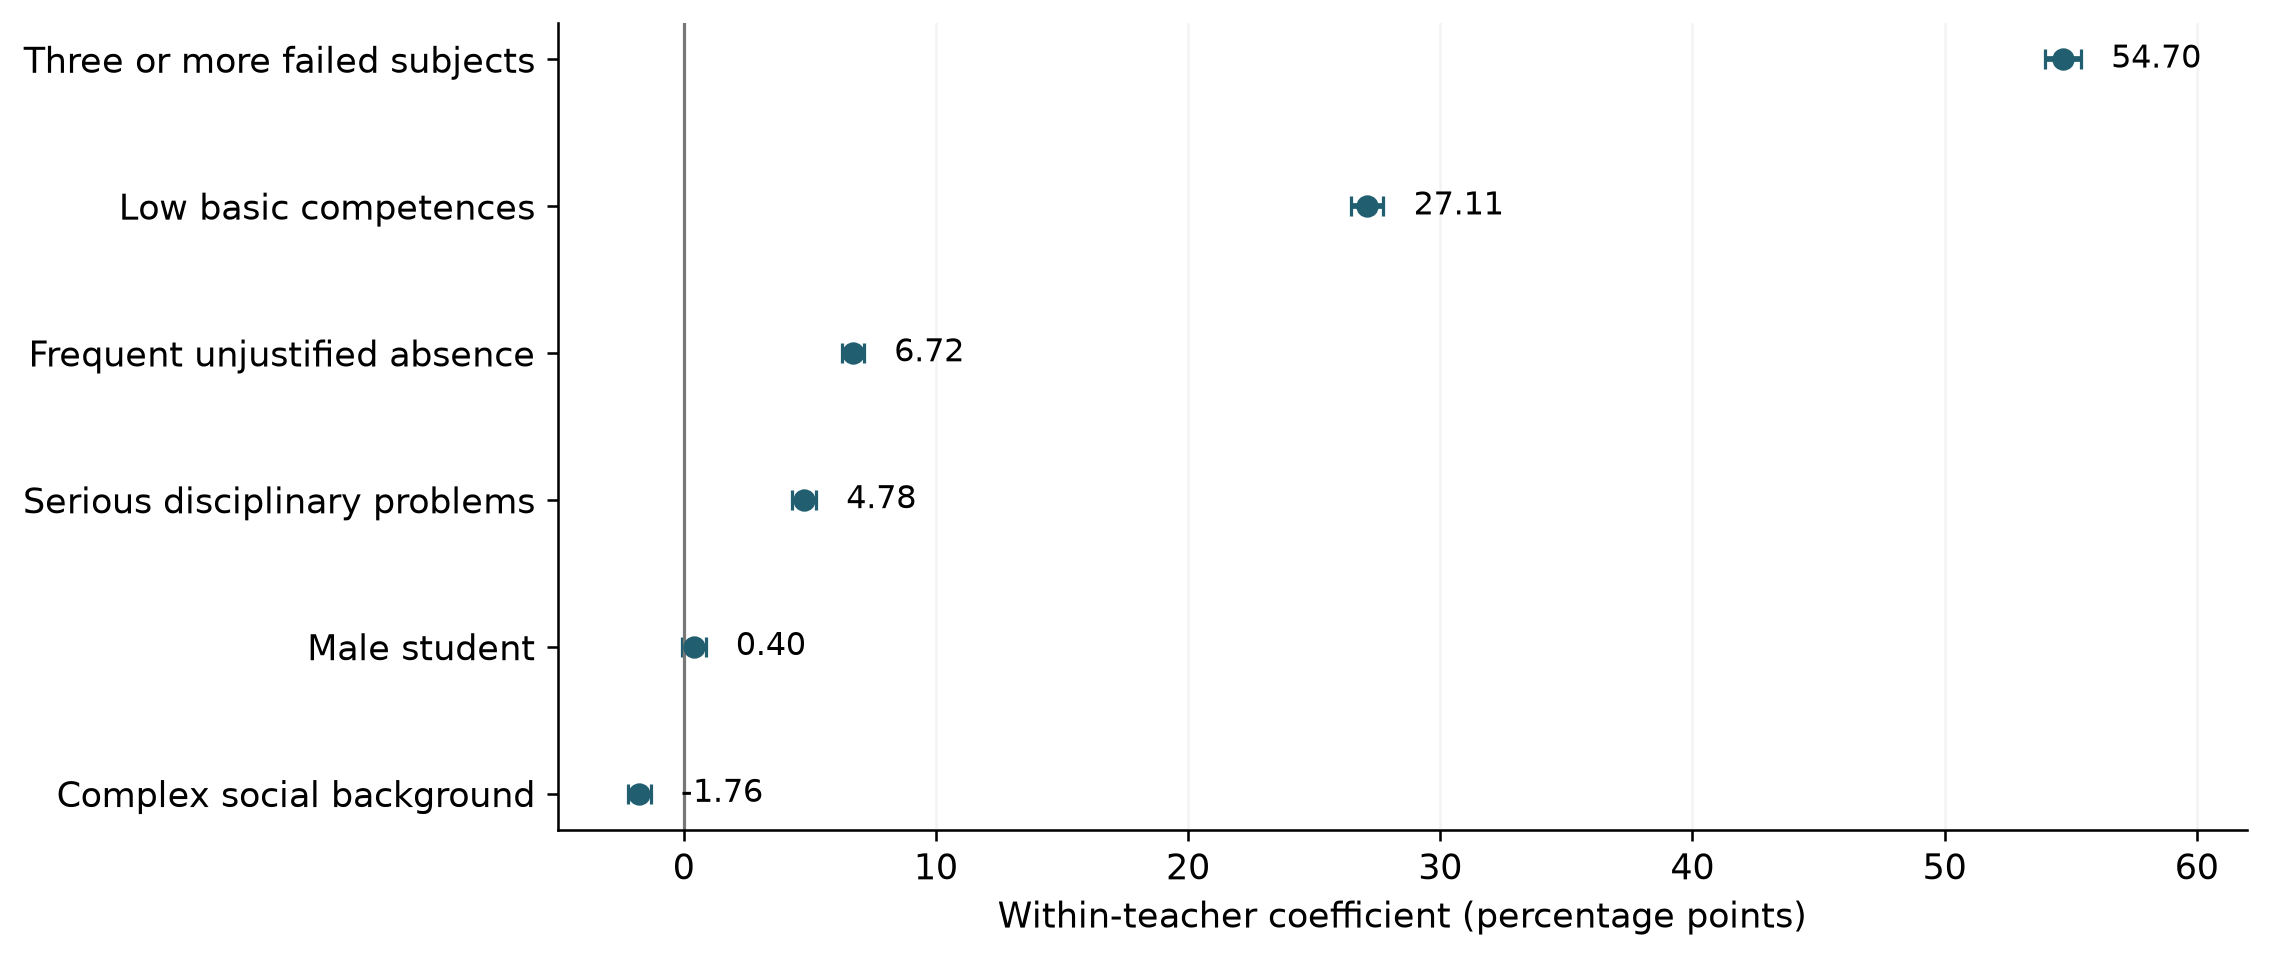
\includegraphics[width=.94\linewidth]{../../3. Output/paper_A/figures/attribute_coefficients.png}
\caption{\textcolor{addedreview}{Within-teacher responses to the six student attributes. Points are percentage-point coefficients; horizontal bars show one teacher-clustered standard error. The vertical line marks zero. Numerical estimates, SE and significance stars are reported in Table~\ref{tab:attr}.}}\label{fig:attributes}
\endgroup\end{figure}


\DIFaddend 



Attendance and conduct retain a role beyond the academic indicators. Frequent unjustified absence adds \DIFdelbegin \DIFdel{6.37 }\DIFdelend \DIFaddbegin \DIFadd{6.72 }\DIFaddend points, and serious disciplinary problems add \DIFdelbegin \DIFdel{4.56 }\DIFdelend \DIFaddbegin \DIFadd{4.78 }\DIFaddend points. Their smaller magnitudes do not make them incidental controls: teachers incorporate information about \DIFdelbegin \DIFdel{the student's }\DIFdelend engagement and behavior when deciding between promotion and repetition. The coefficients alone do not distinguish \DIFdelbegin \DIFdel{whether this reflects }\DIFdelend expected educational gains, perceived readiness or normative considerations about conduct.

Student gender makes little difference to the average recommendation: the male-student coefficient is only \DIFdelbegin \DIFdel{0.26 }\DIFdelend \DIFaddbegin \DIFadd{0.40 }\DIFaddend percentage points and is not statistically distinguishable from zero. A complex social background reduces repetition recommendations by \DIFdelbegin \DIFdel{1.88 }\DIFdelend \DIFaddbegin \DIFadd{1.76 }\DIFaddend points. These results contrast with the higher population incidence of repetition among boys and disadvantaged students \citep{oecd}. They are compatible with some disparities arising from the academic and school circumstances students bring to the promotion decision, rather than an additional penalty attached directly to their group. The background result is also compatible with teachers taking difficult circumstances into account in a compensatory way. This comparison concerns judgments on otherwise comparable profiles, not the full educational process through which population gaps arise.

The interaction specification in Table~\ref{tab:interactions} shows that failed subjects and low competences reinforce one another. Low competences add \DIFdelbegin \DIFdel{about 22 }\DIFdelend \DIFaddbegin \DIFadd{21.45 }\DIFaddend percentage points when the failed-subject indicator is absent and \DIFdelbegin \DIFdel{32 points }\DIFdelend \DIFaddbegin \DIFadd{32.52 }\DIFaddend when it is present\DIFdelbegin \DIFdel{; the interaction remains significant after adjustment for }\DIFdelend \DIFaddbegin \DIFadd{, a difference of 11.07 points that survives Holm adjustment across }\DIFaddend the three interaction tests. \DIFdelbegin \DIFdel{Interactions }\DIFdelend \DIFaddbegin \DIFadd{The interaction }\DIFaddend of failures with \DIFdelbegin \DIFdel{attendance or discipline are smaller and }\DIFdelend \DIFaddbegin \DIFadd{discipline is smaller (2.18 points) but also survives this adjustment; the attendance interaction is }\DIFaddend imprecise. Thus \DIFdelbegin \DIFdel{teachers respond especially strongly when both academic signals indicate difficulty}\DIFdelend \DIFaddbegin \DIFadd{combining academic difficulties produces the strongest reinforcement, alongside a more modest additional role for discipline when subjects are failed}\DIFaddend . The next section examines \DIFdelbegin \DIFdel{what happens when those }\DIFdelend \DIFaddbegin \DIFadd{cases in which academic }\DIFaddend signals point in different directions.

\DIFdelbegin 
\begin{table}[!htbp]
\centering\begingroup\color{deletedreview}
\caption*{\textcolor{deletedreview}{\textbf{Deleted / superseded --- baseline Table 2.} Combining academic and behavioral information within teachers}}
\small
\begin{tabular}{lr}
\toprule
Term & Coefficient (SE) \\
\midrule
Male student & \shortstack{0.24\\{\scriptsize (0.45)}} \\
Complex social background & \shortstack{-2.17$^{***}$\\{\scriptsize (0.45)}} \\
Three or more failed subjects & \shortstack{49.57$^{***}$\\{\scriptsize (1.10)}} \\
Low basic competences & \shortstack{21.66$^{***}$\\{\scriptsize (0.79)}} \\
Frequent unjustified absence & \shortstack{5.77$^{***}$\\{\scriptsize (0.55)}} \\
Serious disciplinary problems & \shortstack{2.97$^{***}$\\{\scriptsize (0.67)}} \\
Failures $\times$ low competences & \shortstack{10.56$^{***}$\\{\scriptsize (1.22)}} \\
Failures $\times$ absence & \shortstack{-0.83\\{\scriptsize (0.85)}} \\
Failures $\times$ discipline & \shortstack{0.38\\{\scriptsize (0.94)}} \\
\bottomrule
\end{tabular}
\tabnote{Teacher fixed effects, 22,006 decisions, 2,587 teachers. Teacher-clustered SE. Stars for the three interactions use Holm-adjusted p-values. All coefficients are percentage points. $^{*}p<.05$, $^{**}p<.01$, $^{***}p<.001$. SE in parentheses.}

\endgroup\end{table}


%DIFDELCMD < 

%DIFDELCMD < 
%DIFDELCMD < 
%DIFDELCMD < %%%
\DIFdelend \subsection{Between teachers: harshness, contested cases and descriptive terciles}
Figure~\ref{fig:harshness} introduces the distribution of harshness. \DIFdelbegin \DIFdel{The adjustment compares each teacher with peers on the same recorded cards. Even though the distribution is allocated around the mean (0), there exists a left tail for teachers that deviate much from their peers by being more lenient. We consider these teachers "non-takers" as they do notsupport grade repetitioneven when facing student cards with high retention rates among their peers}\DIFdelend \DIFaddbegin \DIFadd{Teachers are compared with peers evaluating the same six-attribute profiles. The unweighted teacher mean is close to zero ($-0.12$ percentage points), with a standard deviation of 19.00 points. The lower tail identifies teachers who recommend repetition less often than peers for the profiles they answered; it does not, by itself, establish general opposition to repetition}\DIFaddend .


\DIFdelbegin 
\begin{figure}[!htbp]
\centering\begingroup\color{deletedreview}
\setlength{\fboxsep}{3pt}\fcolorbox{deletedreview}{white}{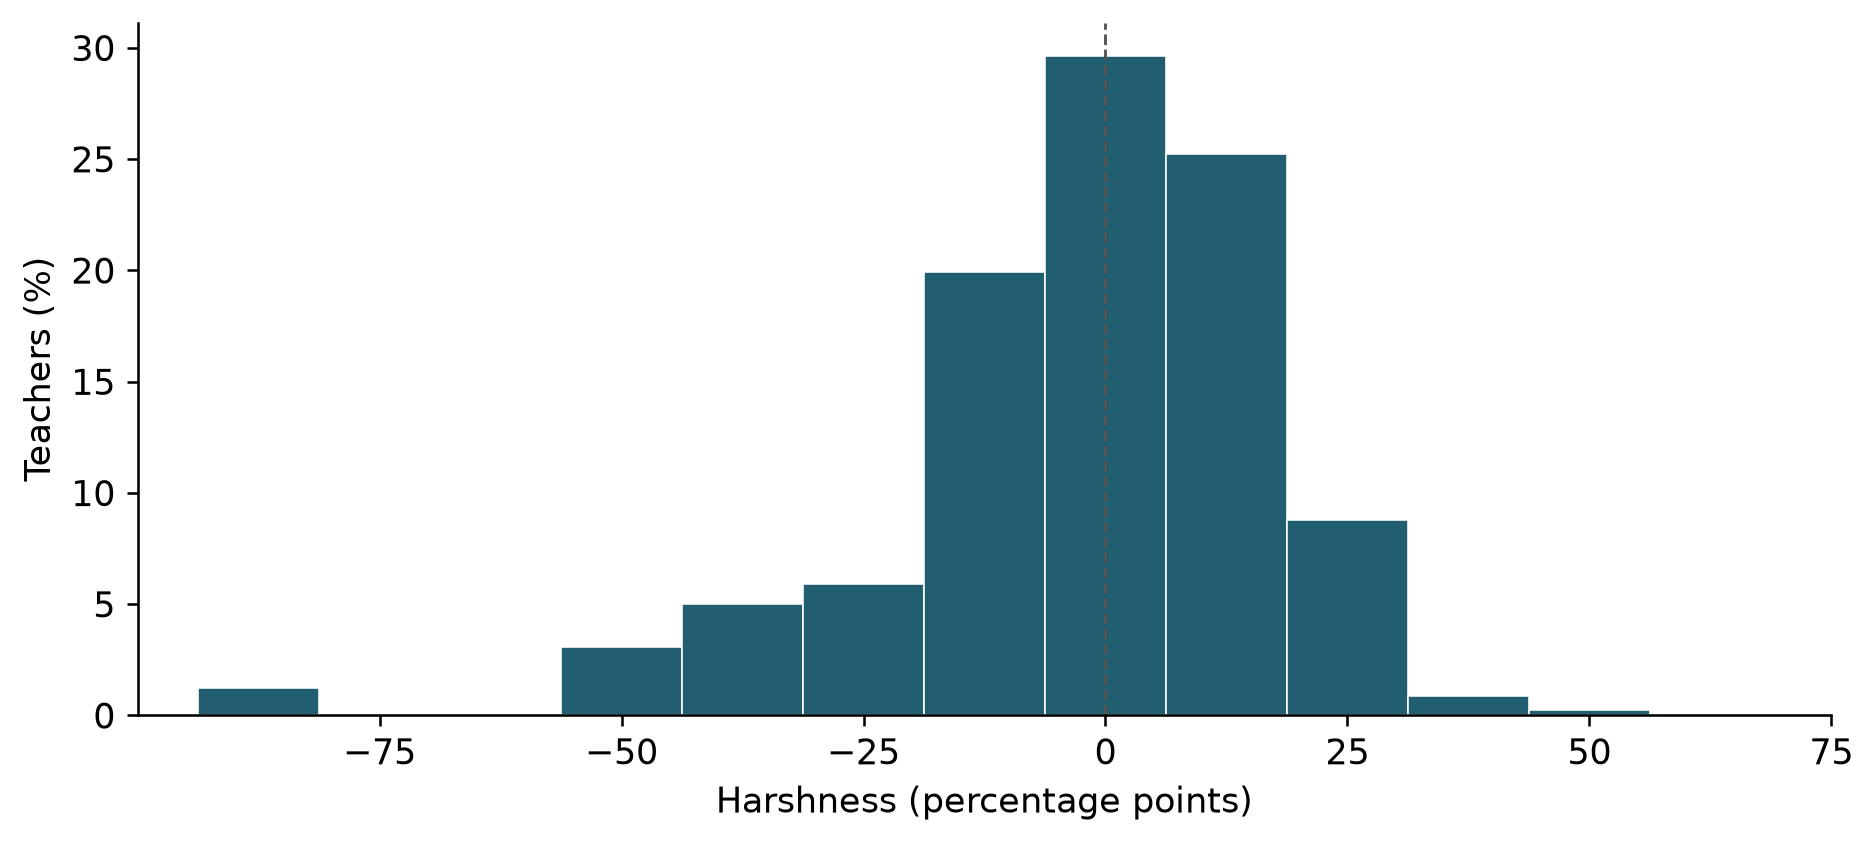
\includegraphics[width=.90\linewidth]{comparison_baseline/harshness_distribution.png}}
\caption*{\textcolor{deletedreview}{\textbf{Deleted / superseded --- baseline Figure 2.} Distribution of harshness among 2,705 teachers, using 12.5-percentage-point bins centered on zero and equal weight per teacher. Negative values indicate fewer repetition recommendations than peers evaluating the same cards; positive values indicate more.}}
\endgroup\end{figure}


\DIFdelend \DIFaddbegin 
\begin{figure}[!htbp]
\centering\begingroup\color{addedreview}
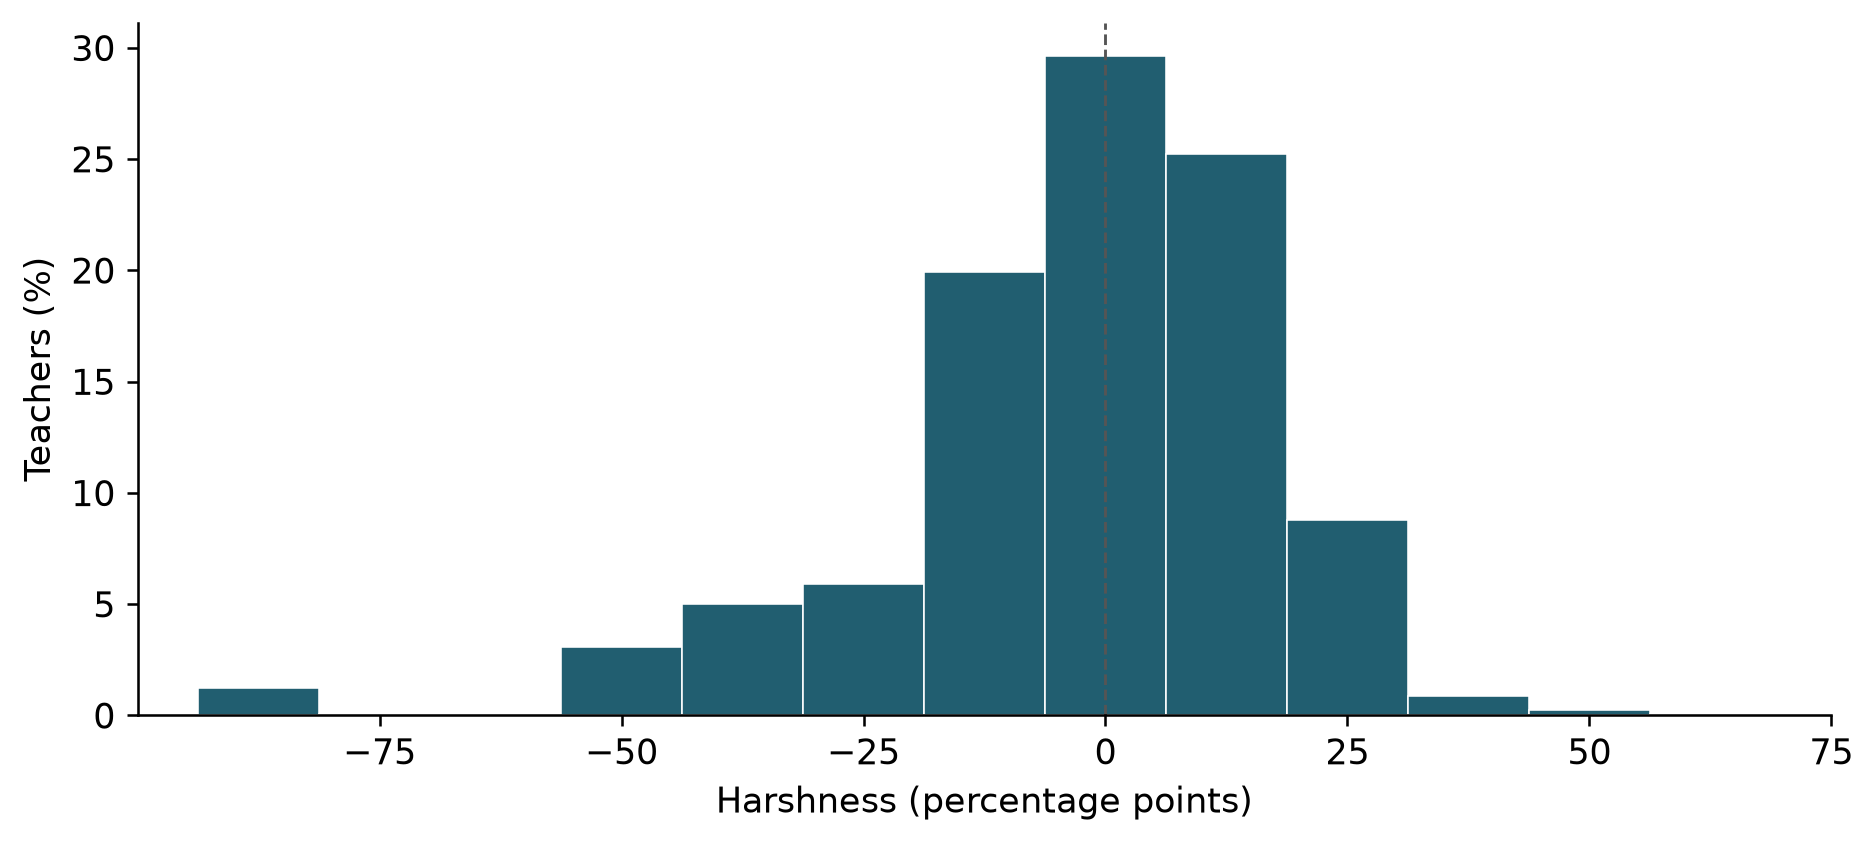
\includegraphics[width=.94\linewidth]{../../3. Output/paper_A/figures/harshness_distribution.png}
\caption{\textcolor{addedreview}{Distribution of harshness among 2,604 teachers, using 12.5-percentage-point bins centered on zero and equal weight per teacher. Negative values indicate fewer repetition recommendations than peers evaluating the same profiles; positive values indicate more.}}\label{fig:harshness}
\endgroup\end{figure}


\DIFaddend 





Same-profile disagreement shows where \DIFdelbegin \DIFdel{teachers' }\DIFdelend judgments diverge. Across \DIFdelbegin \DIFdel{all recorded identifiers}\DIFdelend \DIFaddbegin \DIFadd{the 56 profiles}\DIFaddend , its frequency-weighted value is \DIFdelbegin \DIFdel{25.89 percent. Table~\ref{tab:academic} locates the principal boundary}\DIFdelend \DIFaddbegin \DIFadd{25.22 percent. Figure~\ref{fig:academic} shows the most divided academic category}\DIFaddend : for several failed subjects combined with adequate competences, \DIFdelbegin \DIFdel{the probability that }\DIFdelend two teachers disagree on the same \DIFdelbegin \DIFdel{identifier is 49.11 percent }\DIFdelend \DIFaddbegin \DIFadd{profile in 49.12 percent of pairs}\DIFaddend . When neither academic difficulty is present, disagreement is \DIFdelbegin \DIFdel{only 5.81 }\DIFdelend \DIFaddbegin \DIFadd{5.60 }\DIFaddend percent. Recommendation rates also differ asymmetrically across the \DIFdelbegin \DIFdel{two }\DIFdelend conflicting categories: 51.52 percent for several failures with adequate competences, compared with 23.79 percent for low competences with few failures. \DIFdelbegin \DIFdel{These contrasts explain why a large average response }\DIFdelend \DIFaddbegin \DIFadd{Large average responses }\DIFaddend to academic information \DIFdelbegin \DIFdel{need not produce agreement }\DIFdelend \DIFaddbegin \DIFadd{therefore coexist with disagreement }\DIFaddend when the signals conflict.



\DIFdelbegin 
\begin{table}[!htbp]
\centering\begingroup\color{deletedreview}
\caption*{\textcolor{deletedreview}{\textbf{Deleted / superseded --- baseline Table 3.} Academic profiles and disagreement on the same recorded card}}
\small
\begin{tabular}{p{5.5cm}rrr}
\toprule
Failed subjects / competences & Repeat (\%) & SE & Disagree (\%) \\
\midrule
Fewer than three / adequate competence & 3.04 & 0.26 & 5.81 \\
Fewer than three / low competence & 23.79 & 0.77 & 35.60 \\
Three or more / adequate competence & 51.52 & 0.96 & 49.11 \\
Three or more / low competence & 85.54 & 0.55 & 24.67 \\
\bottomrule
\end{tabular}
\tabnote{Observed category rates with teacher-clustered SE. Disagreement compares two distinct teachers evaluating the same identifier and averages those probabilities by identifier frequency within category. Other attributes are not standardized. No zero-mean hypothesis tests are attached to descriptive rates.}

\endgroup\end{table}


\DIFdelend \DIFaddbegin 
\begin{figure}[!htbp]
\centering\begingroup\color{addedreview}
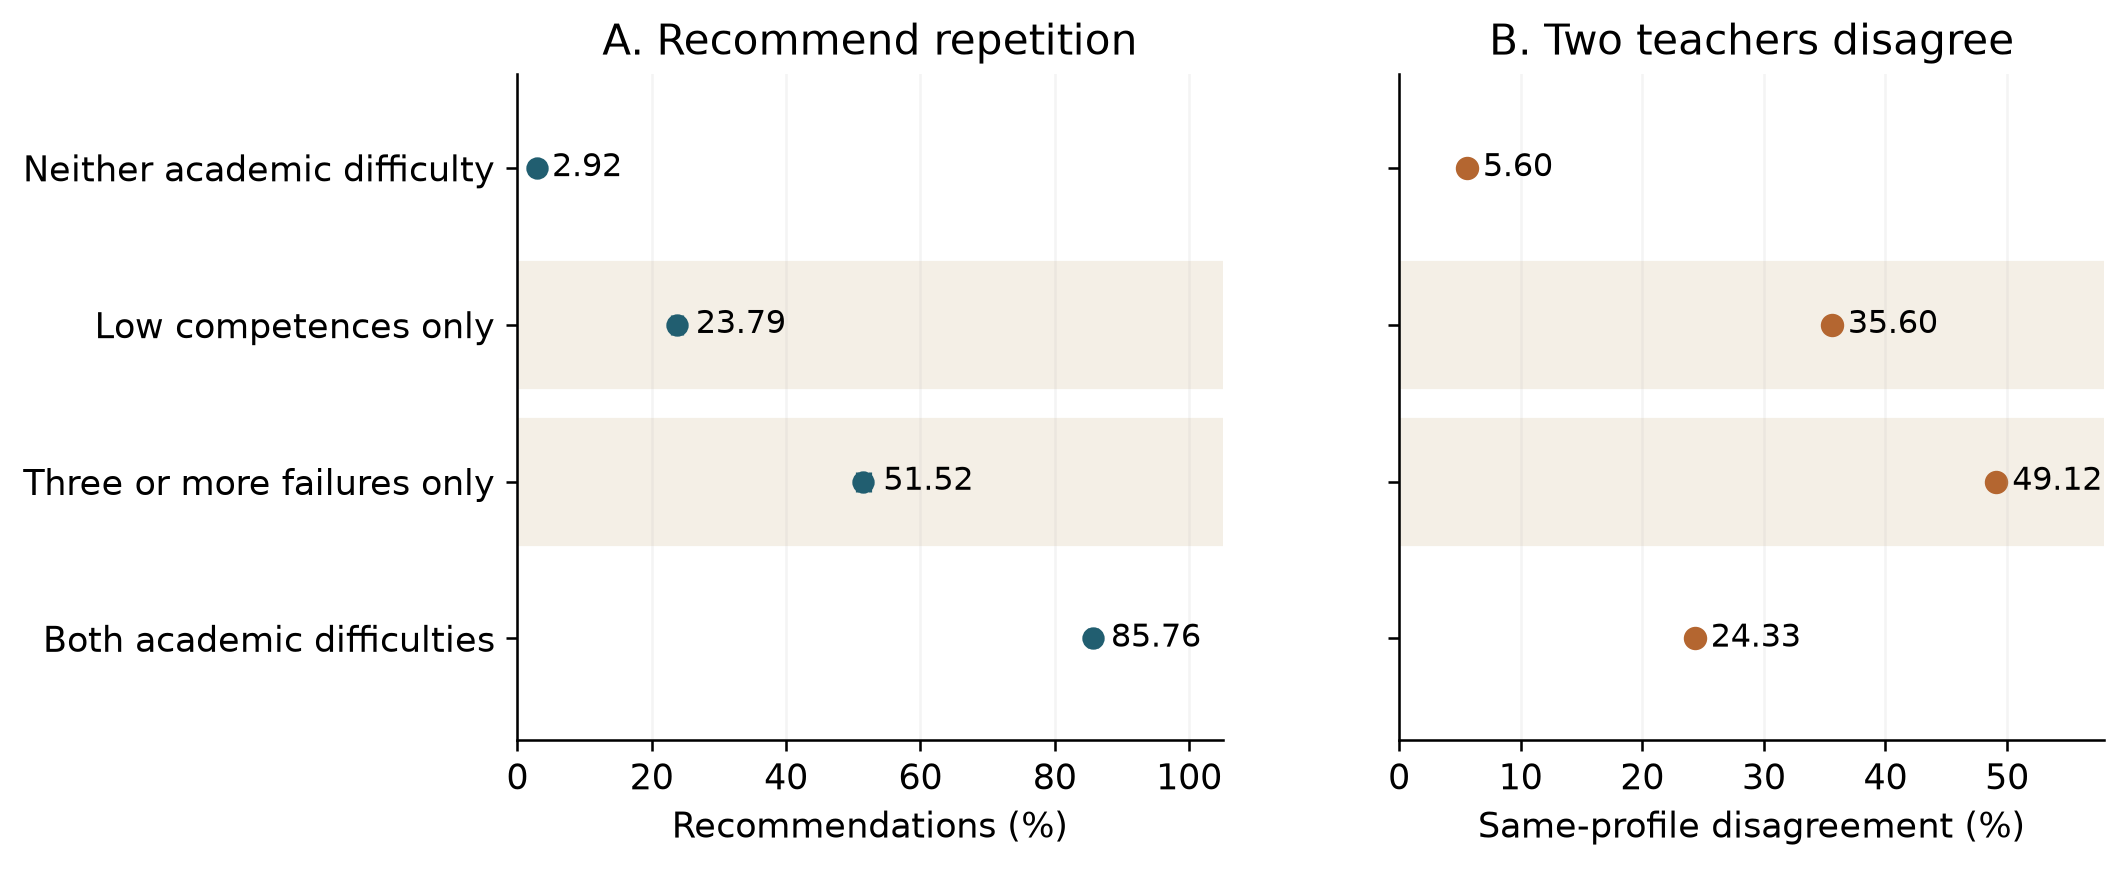
\includegraphics[width=.94\linewidth]{../../3. Output/paper_A/figures/academic_profiles.png}
\caption{\textcolor{addedreview}{Observed repetition recommendations and same-profile disagreement across four combinations of failed subjects and competences. Shaded rows indicate conflicting academic signals. The left panel shows category rates with one teacher-clustered SE; the right shows frequency-weighted disagreement calculated within six-attribute profiles, without uncertainty bars. Remaining attributes are not standardized across categories. Table~\ref{tab:academic} gives the numerical estimates.}}\label{fig:academic}
\endgroup\end{figure}


\DIFaddend 



\DIFaddbegin \DIFadd{Within a profile, pairwise disagreement is greatest when recommendations divide approximately equally. Across a category containing several profiles, however, a repetition rate close to one half can also reflect consensus in opposite directions on different profiles. Computing disagreement within each six-attribute profile distinguishes these possibilities. The high disagreement for failures with adequate competences therefore describes division on comparable cases, rather than only an aggregate balance between repetition and progression.

}

\DIFaddend Tables~\ref{tab:tercsummary} and \ref{tab:tercslopes} \DIFdelbegin \DIFdel{give an accessible description of }\DIFdelend \DIFaddbegin \DIFadd{describe }\DIFaddend differences across the harshness distribution. Teachers in the lower and upper terciles have mean harshness of \DIFdelbegin \DIFdel{$-22.95$ and 18.77 }\DIFdelend \DIFaddbegin \DIFadd{$-20.93$ and 19.36 }\DIFaddend points. Their \DIFdelbegin \DIFdel{observed }\DIFdelend demographic and professional profiles overlap substantially: mean age differs by about two years, and women constitute approximately two-thirds of each group. Secondary teachers account for \DIFdelbegin \DIFdel{43.0 }\DIFdelend \DIFaddbegin \DIFadd{42.9 }\DIFaddend percent of the lower tercile and \DIFdelbegin \DIFdel{53.1 }\DIFdelend \DIFaddbegin \DIFadd{53.7 }\DIFaddend percent of the upper. Agreement that repeaters receive too many resources rises from \DIFdelbegin \DIFdel{3.04 to 4.01 }\DIFdelend \DIFaddbegin \DIFadd{3.06 to 4.02 }\DIFaddend on the 0--10 scale. Effort attribution \DIFdelbegin \DIFdel{, by contrast, }\DIFdelend averages close to seven in all three groups.


\DIFdelbegin 
\begin{table}[!htbp]
\centering\begingroup\color{deletedreview}
\caption*{\textcolor{deletedreview}{\textbf{Deleted / superseded --- baseline Table 4.} Teacher characteristics across observed harshness terciles}}
\small
\begin{tabular}{lrrr}
\toprule
Characteristic & Lower & Middle & Upper \\
\midrule
Teachers & 908 & 864 & 933 \\
Mean harshness (pp) & -22.95 & 1.94 & 18.77 \\
Repetition recommendations (\%) & 25.87 & 48.57 & 70.13 \\
Age (years) & 46.27 & 44.69 & 44.22 \\
Experience (years) & 18.23 & 16.37 & 15.95 \\
Secondary teachers (\%) & 43.0 & 50.9 & 53.1 \\
Female teachers (\%) & 67.6 & 68.2 & 66.3 \\
Effort attribution (1--10) & 7.08 & 7.03 & 7.19 \\
Excess resources (0--10) & 3.04 & 3.55 & 4.01 \\
\bottomrule
\end{tabular}
\tabnote{Terciles use empirical one-third and two-thirds cutoffs of harshness, retaining ties. Characteristic means use available responses within each tercile. Higher repetition shares partly follow from the group definition.}

\endgroup\end{table}


\DIFdelend \DIFaddbegin 
\begin{table}[!htbp]
\centering\begingroup\color{addedreview}
\caption{\textcolor{addedreview}{Teacher characteristics across observed harshness terciles}}\label{tab:tercsummary}
\small
\begin{tabular}{lrrr}
\toprule
Characteristic & Lower & Middle & Upper \\
\midrule
Teachers & 871 & 852 & 881 \\
Mean harshness (pp) & -20.93 & 0.99 & 19.36 \\
Repetition recommendations (\%) & 20.90 & 41.83 & 62.05 \\
Age (years) & 46.42 & 44.63 & 44.04 \\
Experience (years) & 18.19 & 16.52 & 15.66 \\
Secondary teachers (\%) & 42.9 & 50.5 & 53.7 \\
Female teachers (\%) & 68.6 & 67.1 & 67.4 \\
Effort attribution (1--10) & 7.07 & 7.04 & 7.19 \\
Excess resources (0--10) & 3.06 & 3.51 & 4.02 \\
\bottomrule
\end{tabular}
\tabnote{Terciles use empirical one-third and two-thirds cutoffs of harshness, retaining ties. Characteristic means use available responses within each tercile. Higher repetition shares partly follow from the group definition.}

\endgroup\end{table}


\DIFaddend 



\DIFdelbegin \DIFdel{The attribute }\DIFdelend \DIFaddbegin \DIFadd{Attribute }\DIFaddend coefficients differ across these descriptive groups. The failed-subject coefficient is about \DIFdelbegin \DIFdel{33 }\DIFdelend \DIFaddbegin \DIFadd{32 }\DIFaddend points in the lower tercile and \DIFdelbegin \DIFdel{65 points }\DIFdelend \DIFaddbegin \DIFadd{65--67 }\DIFaddend in the other two\DIFdelbegin \DIFdel{, whereas }\DIFdelend \DIFaddbegin \DIFadd{; }\DIFaddend the competence coefficient stays between \DIFdelbegin \DIFdel{roughly 25 }\DIFdelend \DIFaddbegin \DIFadd{26 }\DIFaddend and 29 points. Absence \DIFdelbegin \DIFdel{and discipline have clearer positive coefficients in the lower tercile. In the upper tercile, absence is close to zero and discipline has }\DIFdelend \DIFaddbegin \DIFadd{has a positive coefficient in all three terciles, largest in the middle group. Discipline has positive coefficients in the lower and middle groups but }\DIFaddend a negative coefficient \DIFaddbegin \DIFadd{in the upper group}\DIFaddend . Because terciles are formed from the same responses, these regressions describe \DIFdelbegin \DIFdel{the }\DIFdelend observed patterns rather than identifying three distinct teacher types. The continuous analysis below asks whether observed teacher information helps explain the overall differences.


\DIFdelbegin 
\begin{table}[!htbp]
\centering\begingroup\color{deletedreview}
\caption*{\textcolor{deletedreview}{\textbf{Deleted / superseded --- baseline Table 5.} Within-teacher attribute coefficients across harshness terciles}}
\small
\begin{tabular}{lrrr}
\toprule
Attribute & Lower & Middle & Upper \\
\midrule
Three or more failed subjects & \shortstack{33.19$^{***}$\\{\scriptsize (0.86)}} & \shortstack{65.33$^{***}$\\{\scriptsize (1.26)}} & \shortstack{65.25$^{***}$\\{\scriptsize (1.12)}} \\
Low basic competences & \shortstack{27.97$^{***}$\\{\scriptsize (0.89)}} & \shortstack{28.90$^{***}$\\{\scriptsize (1.25)}} & \shortstack{24.97$^{***}$\\{\scriptsize (1.06)}} \\
Frequent unjustified absence & \shortstack{8.74$^{***}$\\{\scriptsize (0.75)}} & \shortstack{9.93$^{***}$\\{\scriptsize (0.61)}} & \shortstack{0.79\\{\scriptsize (0.75)}} \\
Serious disciplinary problems & \shortstack{11.53$^{***}$\\{\scriptsize (0.91)}} & \shortstack{6.70$^{***}$\\{\scriptsize (0.64)}} & \shortstack{-4.23$^{***}$\\{\scriptsize (0.88)}} \\
Male student & \shortstack{0.17\\{\scriptsize (0.77)}} & \shortstack{0.04\\{\scriptsize (0.80)}} & \shortstack{0.87\\{\scriptsize (0.70)}} \\
Complex social background & \shortstack{1.22\\{\scriptsize (0.81)}} & \shortstack{-3.90$^{***}$\\{\scriptsize (0.72)}} & \shortstack{-3.81$^{***}$\\{\scriptsize (0.72)}} \\
\bottomrule
\end{tabular}
\tabnote{Separate within-teacher regressions within observed harshness terciles; coefficients in percentage points and teacher-clustered SE. $^{*}p<.05$, $^{**}p<.01$, $^{***}p<.001$. SE in parentheses.}

\endgroup\end{table}


\DIFdelend \DIFaddbegin 
\begin{table}[!htbp]
\centering\begingroup\color{addedreview}
\caption{\textcolor{addedreview}{Within-teacher attribute coefficients across harshness terciles}}\label{tab:tercslopes}
\small
\begin{tabular}{lrrr}
\toprule
Attribute & Lower & Middle & Upper \\
\midrule
Three or more failed subjects & \shortstack{31.57$^{***}$\\{\scriptsize (0.81)}} & \shortstack{65.05$^{***}$\\{\scriptsize (1.31)}} & \shortstack{66.95$^{***}$\\{\scriptsize (1.08)}} \\
Low basic competences & \shortstack{27.16$^{***}$\\{\scriptsize (0.90)}} & \shortstack{28.56$^{***}$\\{\scriptsize (1.27)}} & \shortstack{25.94$^{***}$\\{\scriptsize (1.06)}} \\
Frequent unjustified absence & \shortstack{6.30$^{***}$\\{\scriptsize (0.68)}} & \shortstack{10.50$^{***}$\\{\scriptsize (0.55)}} & \shortstack{3.41$^{***}$\\{\scriptsize (0.86)}} \\
Serious disciplinary problems & \shortstack{8.70$^{***}$\\{\scriptsize (0.88)}} & \shortstack{8.41$^{***}$\\{\scriptsize (0.62)}} & \shortstack{-2.65$^{**}$\\{\scriptsize (0.90)}} \\
Male student & \shortstack{2.20$^{**}$\\{\scriptsize (0.74)}} & \shortstack{-1.20\\{\scriptsize (0.83)}} & \shortstack{0.81\\{\scriptsize (0.74)}} \\
Complex social background & \shortstack{-0.66\\{\scriptsize (0.82)}} & \shortstack{-3.81$^{***}$\\{\scriptsize (0.76)}} & \shortstack{-1.54$^{*}$\\{\scriptsize (0.73)}} \\
\bottomrule
\end{tabular}
\tabnote{Separate within-teacher regressions within observed harshness terciles; coefficients in percentage points and teacher-clustered SE. $^{*}p<.05$, $^{**}p<.01$, $^{***}p<.001$. SE in parentheses.}

\endgroup\end{table}


\DIFaddend 



\subsection{Teacher characteristics and the decomposition of decisions}
Table~\ref{tab:char} compares models of harshness on \DIFaddbegin \DIFadd{the same }\DIFaddend 2,\DIFdelbegin \DIFdel{157 teachers. The full specification accounts for less than five }\DIFdelend \DIFaddbegin \DIFadd{164 teachers. Professional and demographic characteristics account for 2.58 }\DIFaddend percent of its observed variation\DIFaddbegin \DIFadd{; adding general beliefs raises this to 2.88 percent, and adding agreement about resources raises it to 4.68 percent}\DIFaddend . Secondary teachers are somewhat more severe on average, and older teachers less severe when compared at the same level of experience. Experience itself has a small, uncertain coefficient. These \DIFdelbegin \DIFdel{differences }\DIFdelend \DIFaddbegin \DIFadd{associations }\DIFaddend coexist with substantial overlap between \DIFdelbegin \DIFdel{the groups : knowing a teacher's career profile provides only limited information about their judgments}\DIFdelend \DIFaddbegin \DIFadd{groups and limited overall fit}\DIFaddend .


\DIFdelbegin 
\begin{table}[!htbp]
\centering\begingroup\color{deletedreview}
\caption*{\textcolor{deletedreview}{\textbf{Deleted / superseded --- baseline Table 6.} Observed characteristics associated with harshness}}
\small
\begin{tabular}{p{5.6cm}rrr}
\toprule
Characteristic & $X_1$ & $X_2$ & $X_3$ \\
\midrule
Constant & \shortstack{11.41$^{***}$\\{\scriptsize (2.95)}} & \shortstack{7.34\\{\scriptsize (4.73)}} & \shortstack{4.27\\{\scriptsize (4.70)}} \\
Secondary stage & \shortstack{3.81$^{***}$\\{\scriptsize (0.87)}} & \shortstack{4.00$^{***}$\\{\scriptsize (0.91)}} & \shortstack{3.33$^{***}$\\{\scriptsize (0.91)}} \\
Experience (years) & \shortstack{0.05\\{\scriptsize (0.08)}} & \shortstack{0.05\\{\scriptsize (0.08)}} & \shortstack{0.03\\{\scriptsize (0.08)}} \\
Female teacher & \shortstack{-0.21\\{\scriptsize (0.85)}} & \shortstack{-0.41\\{\scriptsize (0.87)}} & \shortstack{-0.38\\{\scriptsize (0.87)}} \\
Age (years) & \shortstack{-0.32$^{***}$\\{\scriptsize (0.08)}} & \shortstack{-0.33$^{***}$\\{\scriptsize (0.08)}} & \shortstack{-0.30$^{***}$\\{\scriptsize (0.08)}} \\
Public school & \shortstack{0.38\\{\scriptsize (1.49)}} & \shortstack{0.63\\{\scriptsize (1.49)}} & \shortstack{-0.07\\{\scriptsize (1.50)}} \\
Reported permanent public appointment & \shortstack{-0.13\\{\scriptsize (1.10)}} & \shortstack{-0.11\\{\scriptsize (1.10)}} & \shortstack{0.03\\{\scriptsize (1.10)}} \\
Teaching groups & \shortstack{0.07\\{\scriptsize (0.15)}} & \shortstack{0.07\\{\scriptsize (0.15)}} & \shortstack{0.05\\{\scriptsize (0.14)}} \\
Perceived teacher impact (0--10) & -- & \shortstack{0.06\\{\scriptsize (0.28)}} & \shortstack{0.13\\{\scriptsize (0.28)}} \\
Empathy (1--5) & -- & \shortstack{-0.05\\{\scriptsize (0.70)}} & \shortstack{0.05\\{\scriptsize (0.70)}} \\
Effort attribution (1--10) & -- & \shortstack{0.58$^{*}$\\{\scriptsize (0.23)}} & \shortstack{0.40\\{\scriptsize (0.23)}} \\
Excess resources for repeaters (0--10) & -- & -- & \shortstack{0.88$^{***}$\\{\scriptsize (0.15)}} \\
Teachers & 2157 & 2157 & 2157 \\
$R^2$ (\%) & 2.70 & 3.03 & 4.82 \\
\bottomrule
\end{tabular}
\tabnote{Outcome: harshness, in percentage points. HC3 SE. Same 2,157 teachers in every column. Age and experience enter jointly; resource agreement is in original 0--10 units. $^{*}p<.05$, $^{**}p<.01$, $^{***}p<.001$. SE in parentheses. HC3 stars use the asymptotic normal reference.}

\endgroup\end{table}


\DIFdelend \DIFaddbegin 
\begin{table}[!htbp]
\centering\begingroup\color{addedreview}
\caption{\textcolor{addedreview}{Observed characteristics associated with harshness}}\label{tab:char}
\small
\begin{tabular}{p{5.6cm}rrr}
\toprule
Characteristic & \shortstack{Professional /\\demographic} & \shortstack{+ General\\beliefs} & \shortstack{+ Excess\\resources} \\
\midrule
Constant & \shortstack{10.28$^{***}$\\{\scriptsize (2.90)}} & \shortstack{8.24\\{\scriptsize (4.69)}} & \shortstack{5.21\\{\scriptsize (4.66)}} \\
Secondary stage & \shortstack{4.04$^{***}$\\{\scriptsize (0.87)}} & \shortstack{4.10$^{***}$\\{\scriptsize (0.90)}} & \shortstack{3.43$^{***}$\\{\scriptsize (0.90)}} \\
Experience (years) & \shortstack{0.03\\{\scriptsize (0.08)}} & \shortstack{0.03\\{\scriptsize (0.08)}} & \shortstack{0.01\\{\scriptsize (0.08)}} \\
Female teacher & \shortstack{0.09\\{\scriptsize (0.85)}} & \shortstack{-0.09\\{\scriptsize (0.87)}} & \shortstack{-0.07\\{\scriptsize (0.86)}} \\
Age (years) & \shortstack{-0.30$^{***}$\\{\scriptsize (0.08)}} & \shortstack{-0.31$^{***}$\\{\scriptsize (0.08)}} & \shortstack{-0.27$^{***}$\\{\scriptsize (0.08)}} \\
Public school & \shortstack{0.15\\{\scriptsize (1.47)}} & \shortstack{0.33\\{\scriptsize (1.47)}} & \shortstack{-0.39\\{\scriptsize (1.49)}} \\
Reported permanent public appointment & \shortstack{0.25\\{\scriptsize (1.12)}} & \shortstack{0.28\\{\scriptsize (1.12)}} & \shortstack{0.41\\{\scriptsize (1.11)}} \\
Teaching groups & \shortstack{0.04\\{\scriptsize (0.15)}} & \shortstack{0.04\\{\scriptsize (0.15)}} & \shortstack{0.01\\{\scriptsize (0.14)}} \\
Perceived teacher impact (0--10) & -- & \shortstack{-0.10\\{\scriptsize (0.28)}} & \shortstack{-0.03\\{\scriptsize (0.27)}} \\
Empathy (1--5) & -- & \shortstack{-0.17\\{\scriptsize (0.70)}} & \shortstack{-0.08\\{\scriptsize (0.70)}} \\
Effort attribution (1--10) & -- & \shortstack{0.57$^{*}$\\{\scriptsize (0.22)}} & \shortstack{0.39\\{\scriptsize (0.22)}} \\
Excess resources for repeaters (0--10) & -- & -- & \shortstack{0.88$^{***}$\\{\scriptsize (0.15)}} \\
Teachers & 2164 & 2164 & 2164 \\
$R^2$ (\%) & 2.58 & 2.88 & 4.68 \\
\bottomrule
\end{tabular}
\tabnote{Outcome: harshness, in percentage points. HC3 SE. Same 2,164 teachers in every column. Age and experience enter jointly; resource agreement is in original 0--10 units. $^{*}p<.05$, $^{**}p<.01$, $^{***}p<.001$. SE in parentheses. HC3 stars use a t reference with residual degrees of freedom.}

\endgroup\end{table}


\DIFaddend 



Agreement that too many resources are devoted to repeaters has the clearest belief association. A five-point difference on the 0--10 scale corresponds to about 4.4 percentage points of harshness. The positive association with effort attribution becomes less precise once resource agreement is included; perceived impact and empathy add little.

The decomposition in Figure~\ref{fig:variance} connects the teacher-level associations to the decisions themselves. Student attributes and their pairwise interactions account for \DIFdelbegin \DIFdel{48.63 }\DIFdelend \DIFaddbegin \DIFadd{47.93 }\DIFaddend percent of model-implied variance. Professional and demographic characteristics contribute 0.18 percent and reported beliefs \DIFdelbegin \DIFdel{0.17 }\DIFdelend \DIFaddbegin \DIFadd{0.18 }\DIFaddend percent. Observed harshness contributes \DIFdelbegin \DIFdel{12.70 }\DIFdelend \DIFaddbegin \DIFadd{12.78 }\DIFaddend percent, while differences in teachers' attribute sensitivities contribute a further \DIFdelbegin \DIFdel{17.10 }\DIFdelend \DIFaddbegin \DIFadd{18.80 }\DIFaddend percent. The remaining decision-level component is \DIFdelbegin \DIFdel{21.22 }\DIFdelend \DIFaddbegin \DIFadd{20.12 }\DIFaddend percent.

The distinction between overall severity and criteria matters substantively. Teachers can recommend repetition equally often relative to comparable cases while reacting differently to absence, discipline or academic difficulties. The sensitivity component captures such differences jointly across all six attributes. It does not imply that each attribute contributes equally or that the small mean gender coefficient conceals a particular direction of individual responses.


\DIFdelbegin 
\begin{figure}[!htbp]
\centering\begingroup\color{deletedreview}
\setlength{\fboxsep}{3pt}\fcolorbox{deletedreview}{white}{\includegraphics[width=.90\linewidth]{comparison_baseline/variance_partition.png}}
\caption*{\textcolor{deletedreview}{\textbf{Deleted / superseded --- baseline Figure 3.} Model-based allocation of variation in recorded recommendations. Shares sum to 100 percent under the allocation defined in Equations~\ref{eq:decomposition}--\ref{eq:variance_total}. The lower panel reports estimates and one teacher-bootstrap standard error, based on 199 resamples. Harshness is constructed from the observed decisions; the total represented share of 78.78 percent describes within-sample structure.}}
\endgroup\end{figure}


\DIFdelend \DIFaddbegin 
\begin{figure}[!htbp]
\centering\begingroup\color{addedreview}
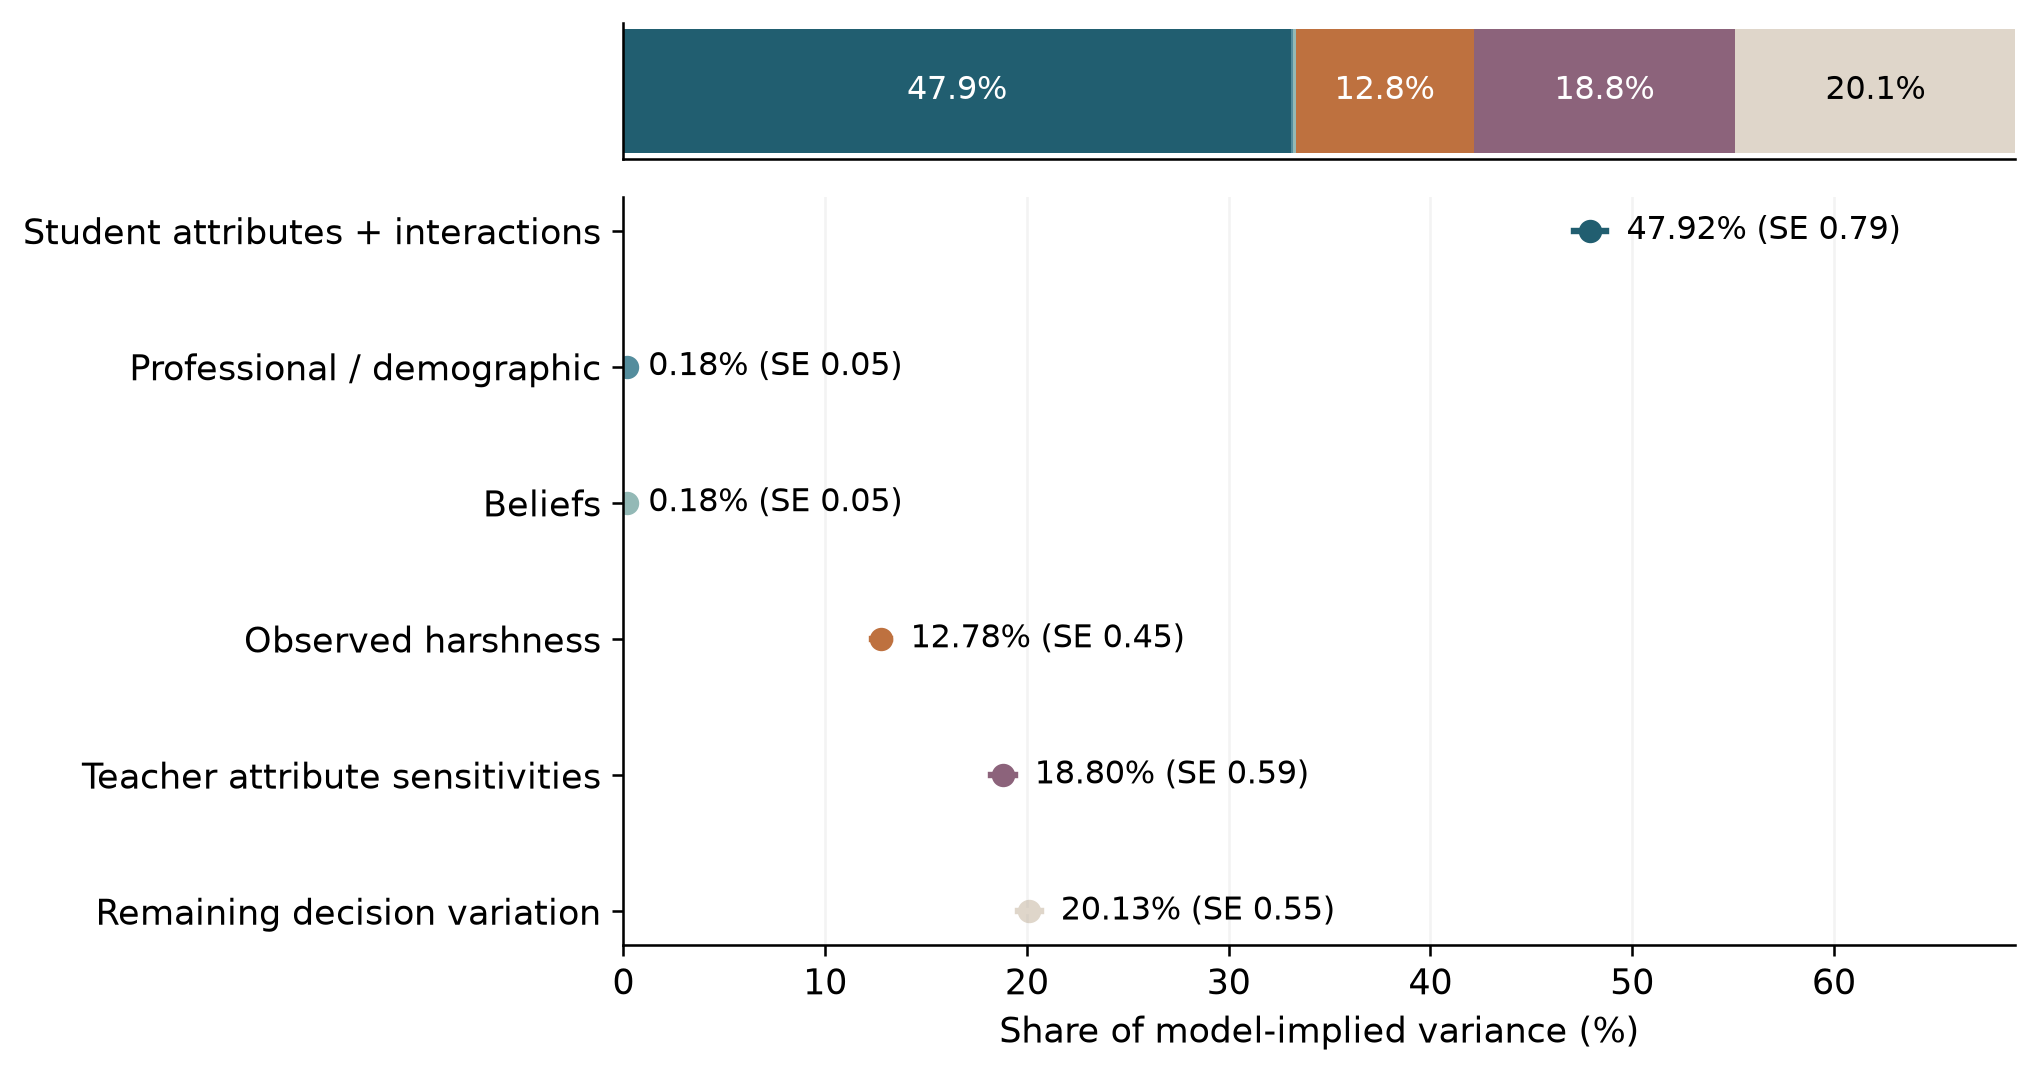
\includegraphics[width=.94\linewidth]{../../3. Output/paper_A/figures/variance_partition.png}
\caption{\textcolor{addedreview}{Model-based allocation of variation in recorded recommendations. Shares sum to 100 percent under the allocation defined in Equations~\ref{eq:decomposition}--\ref{eq:variance_total}. The lower panel reports estimates and one teacher-bootstrap standard error, based on 199 resamples. Harshness is constructed from the observed decisions; the total represented share of 79.88 percent describes within-sample structure.}}\label{fig:variance}
\endgroup\end{figure}


\DIFaddend 


Together, measured information and teacher-specific response patterns represent \DIFdelbegin \DIFdel{78.78 }\DIFdelend \DIFaddbegin \DIFadd{79.88 }\DIFaddend percent of model-implied variance. This is a description of what the complete model captures, including harshness extracted from the same answers. It therefore complements the small teacher-characteristic associations without treating the increase as an improvement in prediction for new teachers.


\DIFaddbegin \DIFadd{The principal pattern survives the reconstruction checks in Table~\ref{tab:reconstruction}. Excluding shared example fields assigns 46.94 percent to student information, 13.24 percent to harshness and 19.29 percent to sensitivities. Omitting the favorable-example screen has a larger effect: the student-information share falls to 44.65 percent and harshness rises to 14.70 percent. These are changes in the descriptive allocation for different samples; the quotas depend on screening as well as on the covariance specification.

}

\DIFaddend \section{Discussion}
The findings connect common criteria with different applications of those criteria. Academic information dominates the average recommendation, but failed subjects and competences are not interchangeable. Their joint presence strengthens the recommendation to repeat, while several failed subjects with adequate competences leave teachers especially divided. The conceptual distinction between diagnosing difficulty and choosing a response helps interpret this boundary: agreement about a student's problems need not entail agreement that another year in the same grade is beneficial.

Attendance, discipline and background extend this account beyond grades. \DIFdelbegin \DIFdel{Their coefficients show that teachers consider more than the two academic indicators. In particular, the }\DIFdelend \DIFaddbegin \DIFadd{The role of conduct is consistent with evidence that behavior enters teachers' grading and promotion judgments \mbox{%DIFAUXCMD
\citep{ferman}}\hskip0pt%DIFAUXCMD
, although our coefficients do not identify whether teachers expect educational gains or apply normative criteria. The }\DIFaddend negative complex-background coefficient is compatible with teachers taking the costs of repetition into account\DIFdelbegin \DIFdel{, even when a difficult context also warrants concern. The contrast with population gender and social disparities makes clear why recommendations on comparable cases and aggregate repetition gaps answer different questions}\DIFdelend . \DIFaddbegin \DIFadd{It need not conflict with less favorable grading of identical work attributed to low-SES students \mbox{%DIFAUXCMD
\citep{doyle}}\hskip0pt%DIFAUXCMD
: the stated background and the decision being evaluated differ. Likewise, evidence connecting gender differences in grading to subsequent achievement \mbox{%DIFAUXCMD
\citep{terrier} }\hskip0pt%DIFAUXCMD
can coexist with our small average gender coefficient in retention recommendations conditional on the information shown. These comparisons distinguish judgments on comparable profiles from the full process generating population disparities.

}\DIFaddend 

Harshness supplies a common measure for describing teacher differences and assessing what observed information captures. Its distribution and descriptive terciles show overall dispersion and variation in attribute associations. The multilevel analysis separates this overall severity from differences in the weight attached to individual attributes. Measured teacher characteristics and beliefs capture little variation, but patterns visible in teachers' decisions account for appreciably more.

The results also delimit what can be inferred from observed teacher profiles. Associations with educational stage, age and resource agreement are present, but substantial individual differences remain within those categories. These descriptors alone do not offer a strong basis for singling out particular teachers. The decomposition directs attention to the criteria applied to student information as well as the overall tendency to recommend repetition. More specific measures of perceived benefits, costs and alternatives might be more closely aligned with the decision framework than broad self-reports; the current data do not establish what those additional measures would explain.

The design's main strength is the comparison of standardized information. Administrative classroom rates mix student sorting and teacher judgment, and some teachers may encounter little variation in particular attributes. The vignette task makes selected contrasts available within teachers and identical profiles available across teachers. Its scope is recommendations under limited stated information. Participation is voluntary, and the regional composition comparison shows overrepresentation of public-school teachers and middle age groups. Final belief availability is also selective. 

The substantive implication is that clarifying promotion decisions may require attention to the interpretation of conflicting information and to the perceived educational response, not only agreement that academic difficulties matter.

\enlargethispage{2\baselineskip}
\section{Conclusion}
Student information strongly organizes teachers' repetition recommendations. Failed subjects and low competences dominate, attendance and discipline add information, and complex social background moderates recommendations. Yet comparable information leaves considerable disagreement, particularly when grades and competences conflict. Observed professional characteristics and beliefs explain little of the differences in harshness. The decision-level decomposition shows that both overall harshness and differences in teachers' responses to individual attributes contribute to the structure of recommendations. Understanding disagreement therefore requires attention to how teachers interpret and combine student information, alongside the information itself.

\clearpage\color{black}\begin{thebibliography}{99}\small\setstretch{1.0}\setlength{\itemsep}{5pt}
\bibitem[Allen et al.(2009)]{allen}  Allen, C. S., Chen, Q., Willson, V. L., \& Hughes, J. N. (2009). Quality of research design moderates effects of grade retention on achievement: A meta-analytic, multilevel analysis. \textit{Educational Evaluation and Policy Analysis, 31}(4), 480--499. \url{https://doi.org/10.3102/0162373709352239}
\bibitem[Bonvin(2003)]{bonvin}  Bonvin, P. (2003). The role of teacher attitudes and judgement in decision-making: The case of grade retention. \textit{European Educational Research Journal, 2}(2), 277--294. \url{https://doi.org/10.2304/eerj.2003.2.2.6}
\DIFaddbegin \bibitem[Bra\~nas-Garza \& Jorrat(2025)]{branasjorrat} \DIFadd{Bra\~nas-Garza, P., \& Jorrat, D. (2025). La repetici\'on perjudica la inclusi\'on social en la escuela. }\textit{\DIFadd{Revista de Educaci\'on, 409}}\DIFadd{, 28--58. }\url{https://doi.org/10.4438/1988-592X-RE-2025-409-685}
\DIFaddend \bibitem[Davoudzadeh et al.(2015)]{davoudzadeh2015readiness}  Davoudzadeh, P., McTernan, M. L., \& Grimm, K. J. (2015). Early school readiness predictors of grade retention from kindergarten through eighth grade: A multilevel discrete-time survival analysis approach. \textit{Early Childhood Research Quarterly, 32}, 183--192. \url{https://doi.org/10.1016/j.ecresq.2015.04.005}
\DIFaddbegin \bibitem[Doyle et al.(2023)]{doyle} \DIFadd{Doyle, L., Easterbrook, M. J., \& Harris, P. R. (2023). Roles of socioeconomic status, ethnicity and teacher beliefs in academic grading. }\textit{British Journal of Educational Psychology, 93}(1)\DIFadd{, 91--112. }\url{https://doi.org/10.1111/bjep.12541}
\bibitem[Ferman \& Fontes(2022)]{ferman} \DIFadd{Ferman, B., \& Fontes, L. F. (2022). Assessing knowledge or classroom behavior? Evidence of teachers' grading bias. }\textit{\DIFadd{Journal of Public Economics, 216}}\DIFadd{, Article 104773. }\url{https://doi.org/10.1016/j.jpubeco.2022.104773}
\bibitem[Garijo-Campos et al.(2025)]{registry}  \DIFadd{Garijo-Campos, I., Alfonso, A., Jorrat, D., Sanchez, A., \& Bra\~nas-Garza, P. (2025). }\textit{\DIFadd{Exploring teachers repetition biases with a survey experiment}} [\DIFadd{AEA RCT Registry, AEARCTR-0015120, version 1.0}]\DIFadd{. }\url{https://doi.org/10.1257/rct.15120-1.0}
\DIFaddend \bibitem[Gonz\'alez-Betancor \& L\'opez-Puig(2016)]{gonzalezbetancor2016retention}  Gonz\'alez-Betancor, S. M., \& L\'opez-Puig, A. J. (2016). Grade retention in primary education is associated with quarter of birth and socioeconomic status. \textit{PLOS ONE, 11}(11), Article e0166431. \url{https://doi.org/10.1371/journal.pone.0166431}
\bibitem[Goos et al.(2021)]{goos}  Goos, M., Pipa, J., \& Peixoto, F. (2021). Effectiveness of grade retention: A systematic review and meta-analysis. \textit{Educational Research Review, 34}, Article 100401. \url{https://doi.org/10.1016/j.edurev.2021.100401}
\bibitem[Gr\"omping(2006)]{groemping}  Gr\"omping, U. (2006). Relative importance for linear regression in R: The package relaimpo. \textit{Journal of Statistical Software, 17}(1), 1--27. \url{https://doi.org/10.18637/jss.v017.i01}
\bibitem[Hainmueller et al.(2014)]{conjoint}  Hainmueller, J., Hopkins, D. J., \& Yamamoto, T. (2014). Causal inference in conjoint analysis: Understanding multidimensional choices via stated preference experiments. \textit{Political Analysis, 22}(1), 1--30. \url{https://doi.org/10.1093/pan/mpt024}
\bibitem[Klapproth \& Beyte(2026)]{klapproth}  Klapproth, F., \& Beyte, C. (2026). GPA, student gender, school subject, and teacher attitudes in grade retention decisions: An experimental study. \textit{European Journal of Psychology of Education, 41}, Article 24. \url{https://doi.org/10.1007/s10212-026-01072-7}
\bibitem[Klapproth \& Schaltz(2015)]{klapprothschaltz2015retained}  Klapproth, F., \& Schaltz, P. (2015). Who is retained in school, and when? Survival analysis of predictors of grade retention in Luxembourgish secondary school. \textit{European Journal of Psychology of Education, 30}(1), 119--136. \url{https://doi.org/10.1007/s10212-014-0232-7}
\bibitem[Mattison et al.(2018)]{mattison2018behavior}  Mattison, A., Raffaele Mendez, L. M., Dedrick, R., Dickinson, S., Wingate, E., \& Hanks, C. (2018). Early elementary teacher ratings of behavior as predictors of grade retention: Race, gender, and socioeconomic status as potential moderators. \textit{Psychology in the Schools, 55}(10), 1171--1187. \url{https://doi.org/10.1002/pits.22192}
\bibitem[Nakagawa et al.(2017)]{nakagawa}  Nakagawa, S., Johnson, P. C. D., \& Schielzeth, H. (2017). The coefficient of determination $R^2$ and intra-class correlation coefficient from generalized linear mixed-effects models revisited and expanded. \textit{Journal of the Royal Society Interface, 14}(134), Article 20170213. \url{https://doi.org/10.1098/rsif.2017.0213}
\bibitem[OECD(2023)]{oecd}  OECD. (2023). \textit{PISA 2022 results (Volume II): Learning during---and from---disruption}. OECD Publishing. \url{https://doi.org/10.1787/a97db61c-en}
\bibitem[Pajares(1992)]{pajares}  Pajares, M. F. (1992). Teachers' beliefs and educational research: Cleaning up a messy construct. \textit{Review of Educational Research, 62}(3), 307--332. \url{https://doi.org/10.3102/00346543062003307}
\bibitem[Santos \& Monteiro(2024)]{santosmonteiro2024retention}  Santos, N. N., \& Monteiro, V. (2024). Second grade retention: Beliefs, decision-making styles, and factors involved in the decision process. \textit{Psychology in the Schools, 61}(4), 1646--1666. \url{https://doi.org/10.1002/pits.23130}
\DIFaddbegin \bibitem[Terrier(2020)]{terrier} \DIFadd{Terrier, C. (2020). Boys lag behind: How teachers' gender biases affect student achievement. }\textit{\DIFadd{Economics of Education Review, 77}}\DIFadd{, Article 101981. }\url{https://doi.org/10.1016/j.econedurev.2020.101981}
\DIFaddend \bibitem[Tomchin \& Impara(1992)]{tomchin}  Tomchin, E. M., \& Impara, J. C. (1992). Unraveling teachers' beliefs about grade retention. \textit{American Educational Research Journal, 29}(1), 199--223. \url{https://doi.org/10.3102/00028312029001199}
\DIFaddbegin \bibitem[Valbuena et al.(2021)]{valbuena} \DIFadd{Valbuena, J., Mediavilla, M., Choi, \'A., \& Gil, M. (2021). Effects of grade retention policies: A literature review of empirical studies applying causal inference. }\textit{Journal of Economic Surveys, 35}(2)\DIFadd{, 408--451. }\url{https://doi.org/10.1111/joes.12406}
\DIFaddend \end{thebibliography}

\clearpage\appendix\setstretch{1.05}

\section{Sample, participation and questionnaire progression}\label{app:sample}
Figure~\ref{fig:flow} starts with 4,037 records that reach the teaching-experience question or a later stage. The 905 entries with \DIFdelbegin \DIFdel{only }\DIFdelend minimal initial engagement are set aside before this flow\DIFdelbegin \DIFdel{; some answer only educational stage, grades taught or subject specialization}\DIFdelend . Among the 4,037, 934 stop before recording any card decision. Of the 3,103 \DIFdelbegin \DIFdel{who answer }\DIFdelend \DIFaddbegin \DIFadd{answering }\DIFaddend a card, including examples, 175 do not reach the end of the decision block\DIFdelbegin \DIFdel{. Thirty-one }\DIFdelend \DIFaddbegin \DIFadd{; 31 }\DIFaddend of these also \DIFdelbegin \DIFdel{fail the screening rule}\DIFdelend \DIFaddbegin \DIFadd{meet the screening exclusion}\DIFaddend . Among the 2,928 \DIFdelbegin \DIFdel{who reach }\DIFdelend \DIFaddbegin \DIFadd{reaching }\DIFaddend the end, a further \DIFdelbegin \DIFdel{358 fail the }\DIFdelend \DIFaddbegin \DIFadd{348 meet that }\DIFaddend rule, giving \DIFdelbegin \DIFdel{389 exclusions in total }\DIFdelend \DIFaddbegin \DIFadd{379 exclusions }\DIFaddend without double counting. Of the 2,\DIFdelbegin \DIFdel{570 remaining, 216 }\DIFdelend \DIFaddbegin \DIFadd{580 remaining, 218 }\DIFaddend do not finish the subsequent survey and 2,\DIFdelbegin \DIFdel{354 }\DIFdelend \DIFaddbegin \DIFadd{362 }\DIFaddend finish. These categories describe recorded progression, not respondents' reasons for stopping.


\DIFdelbegin 
\begin{figure}[!htbp]
\centering\begingroup\color{deletedreview}
\setlength{\fboxsep}{3pt}\fcolorbox{deletedreview}{white}{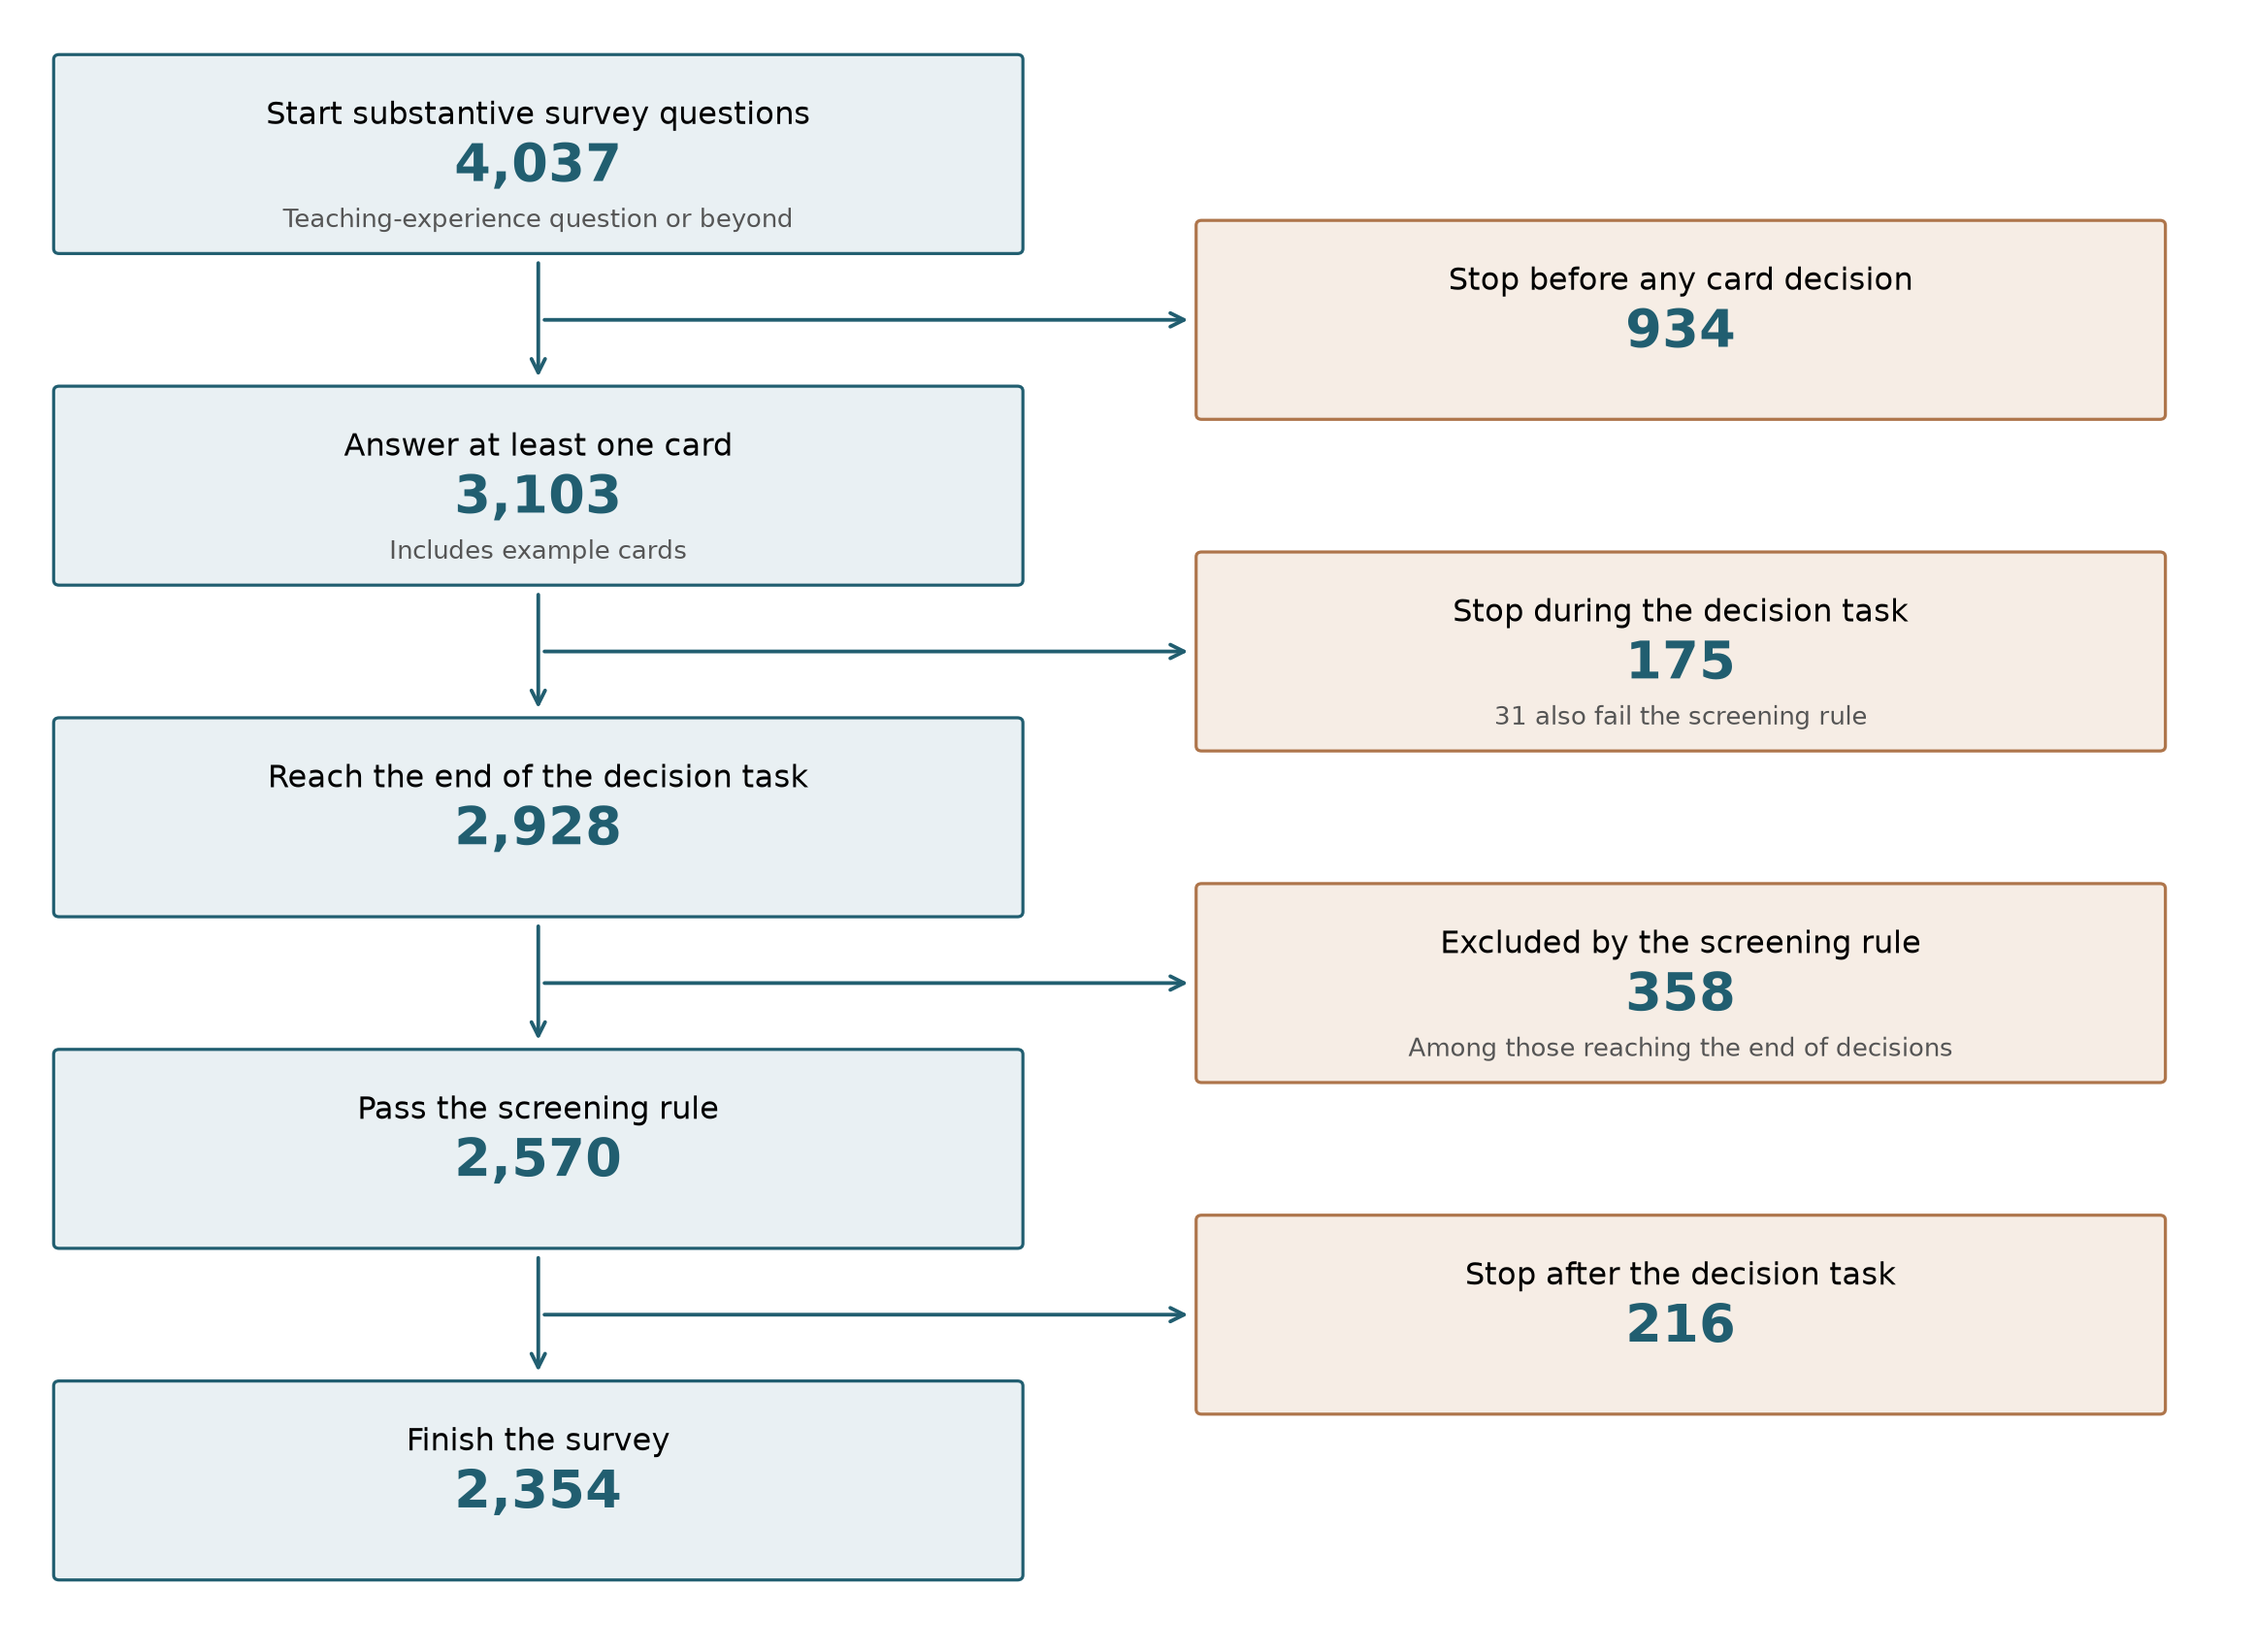
\includegraphics[width=.90\linewidth]{comparison_baseline/sample_flow.png}}
\caption*{\textcolor{deletedreview}{\textbf{Deleted / superseded --- baseline Figure 4.} Participation after excluding 905 entries with minimal initial engagement. Reaching the end of decisions uses the recorded card-block closing flag and does not require an answer to every card. Screening is an analytical exclusion, not necessarily an automatic survey exit.}}
\endgroup\end{figure}


\DIFdelend \DIFaddbegin 
\begin{figure}[!htbp]
\centering\begingroup\color{addedreview}
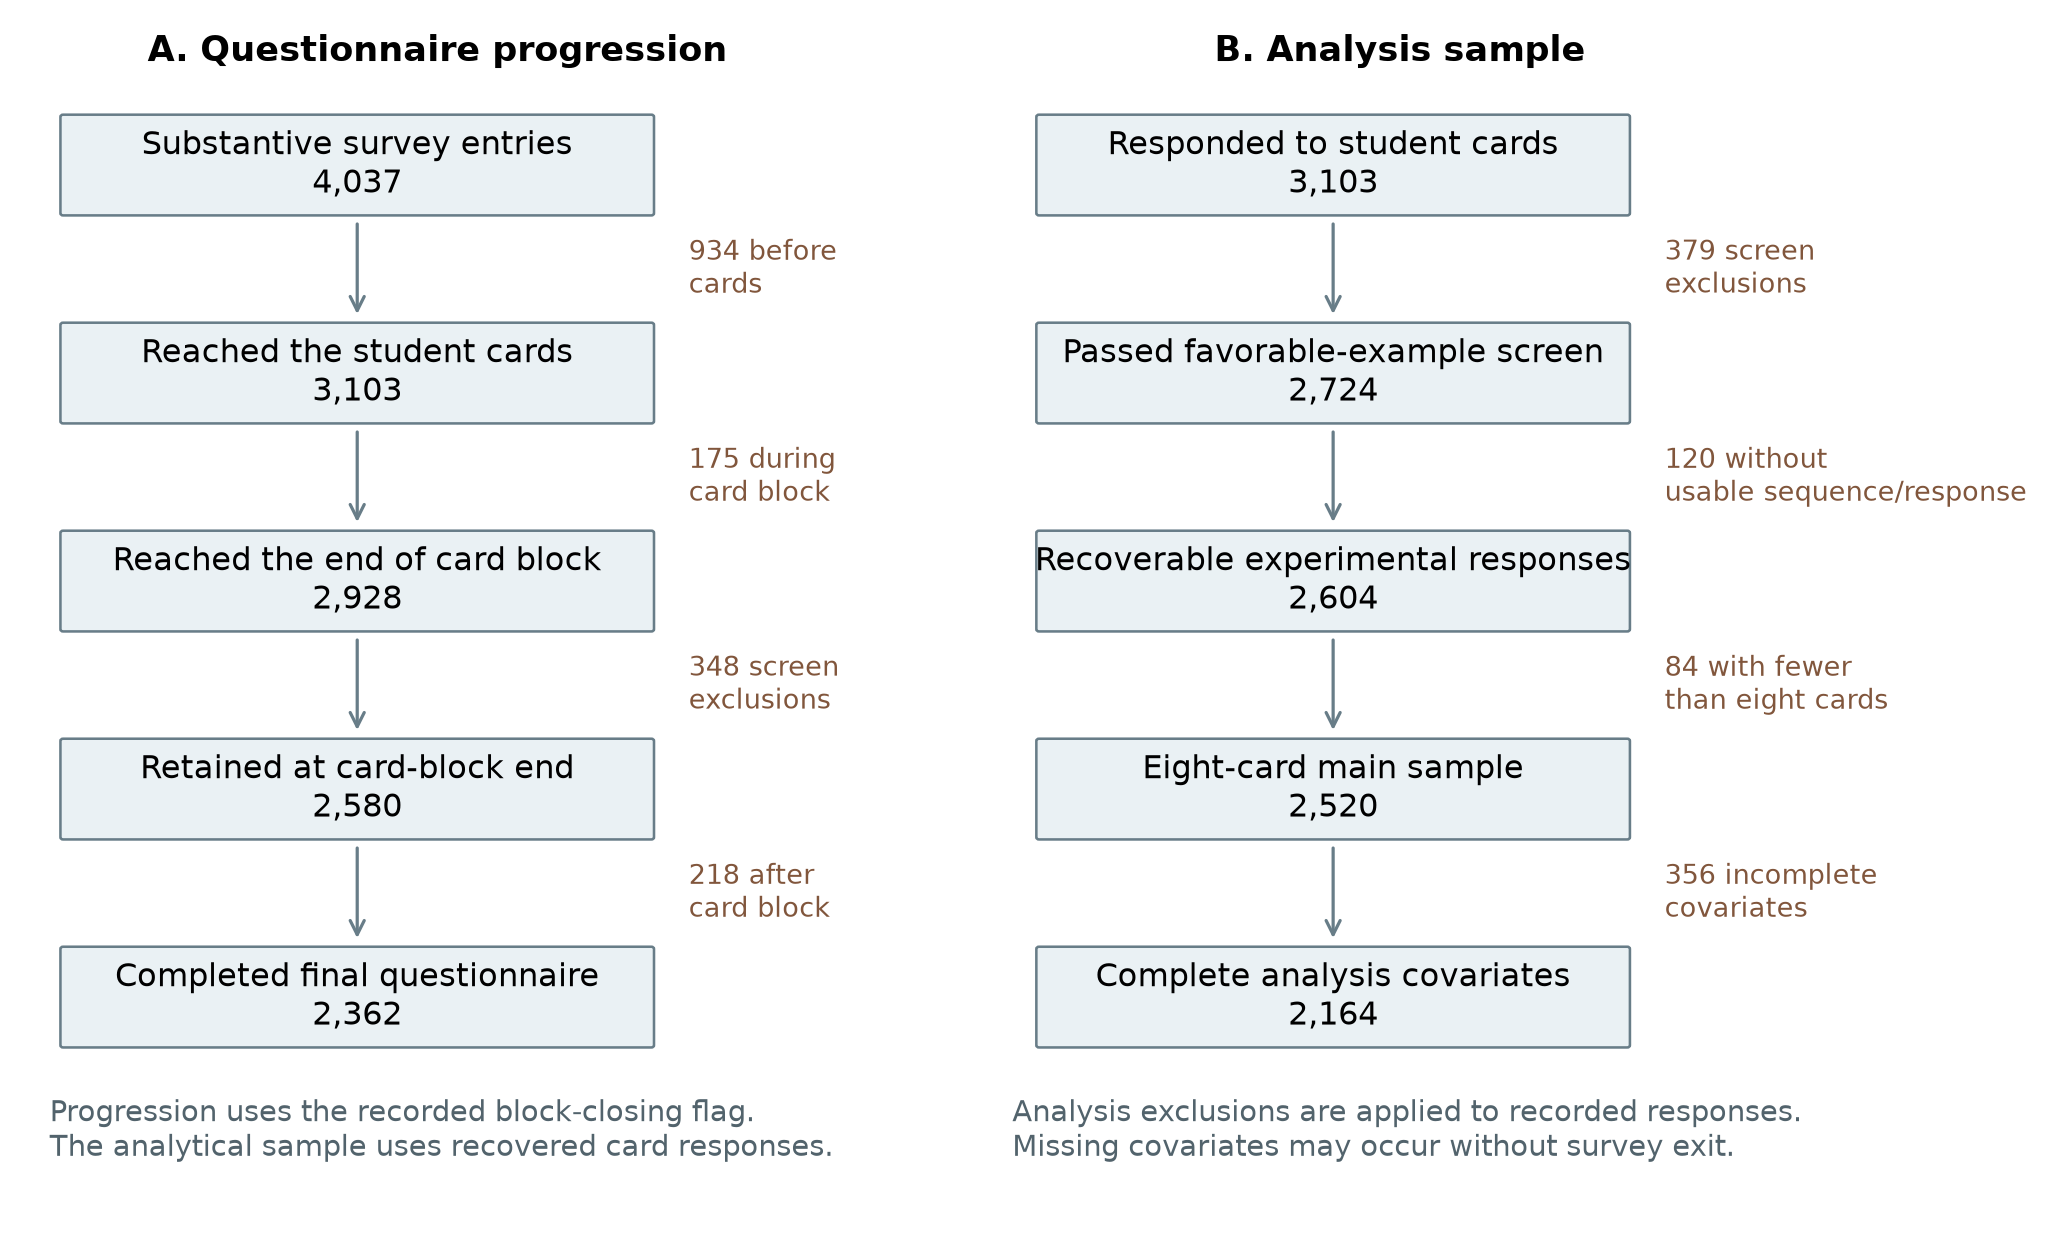
\includegraphics[width=.94\linewidth]{../../3. Output/paper_A/figures/sample_flow.png}
\caption{\textcolor{addedreview}{Participation after excluding 905 entries with minimal initial engagement. Reaching the end of decisions uses the recorded block-closing flag, not completion of all eight cards. Screening is an analytical exclusion.}}\label{fig:flow}
\endgroup\end{figure}


\DIFaddend 



The analytical sample \DIFdelbegin \DIFdel{also retains 135 teachers with usable partial decisions who did not reach the end of the task, giving }\DIFdelend \DIFaddbegin \DIFadd{requires a valid ordered sequence and at least one observed experimental response. Of the }\DIFaddend 2,\DIFdelbegin \DIFdel{705 teachers; nine further partial records contain only fields omitted from the outcome. Among those analyzed }\DIFdelend \DIFaddbegin \DIFadd{580 screened-in records reaching the block end, four have no usable experimental response. Adding 28 usable partial-task records gives 2}\DIFaddend ,\DIFaddbegin \DIFadd{604 teachers. Overall, 120 nonscreened card respondents have no recoverable experimental decision: 102 lack a valid sequence and 18 have no response within that sequence. Among analyzed teachers, }\DIFaddend 2,\DIFdelbegin \DIFdel{203 have }\DIFdelend \DIFaddbegin \DIFadd{520 have eight responses, 84 have fewer, 2,210 have }\DIFaddend all selected belief items and 2,\DIFdelbegin \DIFdel{157 }\DIFdelend \DIFaddbegin \DIFadd{164 }\DIFaddend have all analysis covariates. \DIFdelbegin \DIFdel{A missing covariate does not necessarily }\DIFdelend \DIFaddbegin \DIFadd{Missing covariates need not }\DIFaddend indicate survey exit.


\DIFaddbegin \DIFadd{The eight sets contain eight positions each but only 56 distinct profiles overall. Table~\ref{tab:sets} describes their composition. The reconstruction checks eight distinct assigned identifiers per valid sequence and no duplicate profile within a teacher. Responses outside that sequence are omitted. Harshness references pool matching six-attribute profiles across sets and exclude the focal teacher. Table~\ref{tab:reconstruction} compares reconstruction B with removal of shared fields, no outcome-based screen, complete eight-response records and identifier-specific references.

}




\begin{table}[!htbp]
\centering\begingroup\color{addedreview}
\caption{\textcolor{addedreview}{Composition of the eight assigned sets}}\label{tab:sets}
\small
\begin{tabular}{lrrrrrr}
\toprule
Set & Male & Complex context & Failures & Low competences & Absence & Discipline \\
\midrule
1 & 4 & 4 & 3 & 4 & 4 & 4 \\
2 & 4 & 4 & 3 & 4 & 4 & 4 \\
3 & 4 & 4 & 3 & 4 & 4 & 4 \\
4 & 4 & 4 & 3 & 4 & 4 & 4 \\
5 & 4 & 4 & 5 & 4 & 2 & 3 \\
6 & 4 & 4 & 5 & 4 & 2 & 3 \\
7 & 4 & 4 & 5 & 4 & 2 & 3 \\
8 & 4 & 4 & 5 & 4 & 2 & 3 \\
\bottomrule
\end{tabular}
\tabnote{Number of cards carrying each attribute among the eight assigned positions. Each set contains two cards of each gender-by-background combination. There are 56 distinct profiles across the 64 positions; eight profiles occur twice.}

\endgroup\end{table}








\begin{table}[!htbp]
\centering\begingroup\color{addedreview}
\caption{\textcolor{addedreview}{Reconstruction, screening and reference sensitivities}}\label{tab:reconstruction}
\small
\begin{tabular}{p{3.6cm}rrrrr}
\toprule
Quantity & Main B & No shared & No screen & Eight only & By ID \\
\midrule
Teachers & 2604 & 2597 & 2957 & 2520 & 2604 \\
Decisions & 20467 & 19811 & 23211 & 20160 & 20467 \\
Harshness SD (pp) & 19.00 & 19.30 & 20.53 & 18.54 & 19.01 \\
Harshness $R^2$ (\%) & 4.68 & 4.66 & 3.97 & 4.68 & 4.68 \\
Student information & 47.93 & 46.94 & 44.65 & 47.92 & 47.94 \\
\shortstack[l]{Professional /\\demographic} & 0.18 & 0.19 & 0.10 & 0.18 & 0.18 \\
Beliefs & 0.18 & 0.18 & 0.24 & 0.18 & 0.18 \\
Observed harshness & 12.78 & 13.24 & 14.70 & 12.78 & 12.77 \\
Attribute sensitivities & 18.80 & 19.29 & 19.26 & 18.80 & 18.81 \\
Residual & 20.12 & 20.15 & 21.06 & 20.13 & 20.12 \\
\bottomrule
\end{tabular}
\tabnote{No shared removes experimental positions sharing their response field with that respondent's examples. No screen retains the ordered responses without the favorable-example exclusion. Eight only retains complete eight-answer records. By ID uses original card identifiers rather than pooling identical profiles, on the same B records. The last six rows are variance shares from the same diagonal specification, on each scenario's complete covariate sample.}

\endgroup\end{table}








\begin{table}[!htbp]
\centering\begingroup\color{addedreview}
\caption{\textcolor{addedreview}{Attribute coefficients in pooled and control contexts}}\label{tab:context}
\small
\begin{tabular}{lrr}
\toprule
Attribute & Pooled & Control \\
\midrule
Three or more failed subjects & \shortstack{54.70$^{***}$\\{\scriptsize (0.71)}} & \shortstack{54.28$^{***}$\\{\scriptsize (2.25)}} \\
Low basic competences & \shortstack{27.11$^{***}$\\{\scriptsize (0.63)}} & \shortstack{27.01$^{***}$\\{\scriptsize (1.93)}} \\
Frequent unjustified absence & \shortstack{6.72$^{***}$\\{\scriptsize (0.43)}} & \shortstack{7.78$^{***}$\\{\scriptsize (1.39)}} \\
Serious disciplinary problems & \shortstack{4.78$^{***}$\\{\scriptsize (0.47)}} & \shortstack{6.26$^{***}$\\{\scriptsize (1.49)}} \\
Male student & \shortstack{0.40\\{\scriptsize (0.47)}} & \shortstack{1.59\\{\scriptsize (1.48)}} \\
Complex social background & \shortstack{-1.76$^{***}$\\{\scriptsize (0.45)}} & \shortstack{-0.12\\{\scriptsize (1.42)}} \\
\bottomrule
\end{tabular}
\tabnote{Teacher fixed effects and teacher-clustered SE. Pooled: 20,452 decisions, 2,589 teachers; control: 2,142 decisions, 276 teachers. The comparison checks sensitivity to context restriction; differences in significance are not tests of coefficient differences. $^{*}p<.05$, $^{**}p<.01$, $^{***}p<.001$. SE in parentheses.}

\endgroup\end{table}






\DIFaddend \subsection{Within-task availability and time}
Order fields recover eight distinct \DIFdelbegin \DIFdel{card }\DIFdelend positions for 2,981 raw records, \DIFdelbegin \DIFdel{including records subsequently excluded by screening}\DIFdelend \DIFaddbegin \DIFadd{of which 2,622 pass the favorable-example screen}\DIFaddend . Figure~\ref{fig:progression} \DIFdelbegin \DIFdel{reports the percentage of cards answered and page-submit times by position, omitting six identifiers potentially shared with examples or screening fields. The denominator consists of eligible ordered entries and varies slightlyby position; it is not the initial participation denominator}\DIFdelend \DIFaddbegin \DIFadd{uses nonshared positions within these eligible sequences, excluding a field only when it coincides with that respondent's example. Position-specific denominators therefore differ slightly}\DIFaddend . The percentage answered \DIFdelbegin \DIFdel{decreases from 98.97 }\DIFdelend \DIFaddbegin \DIFadd{falls from 99.02 }\DIFaddend at the first position to \DIFdelbegin \DIFdel{95.98 }\DIFdelend \DIFaddbegin \DIFadd{96.19 }\DIFaddend at the eighth\DIFdelbegin \DIFdel{. Median }\DIFdelend \DIFaddbegin \DIFadd{; median }\DIFaddend positive page-submit \DIFdelbegin \DIFdel{times fall from 16.32 to 10.46 }\DIFdelend \DIFaddbegin \DIFadd{time falls from 16.17 to 10.29 }\DIFaddend seconds. A teacher- and \DIFdelbegin \DIFdel{card-adjusted timing }\DIFdelend \DIFaddbegin \DIFadd{profile-adjusted }\DIFaddend regression also shows faster responses as the task progresses.


\DIFdelbegin 
\begin{figure}[!htbp]
\centering\begingroup\color{deletedreview}
\setlength{\fboxsep}{3pt}\fcolorbox{deletedreview}{white}{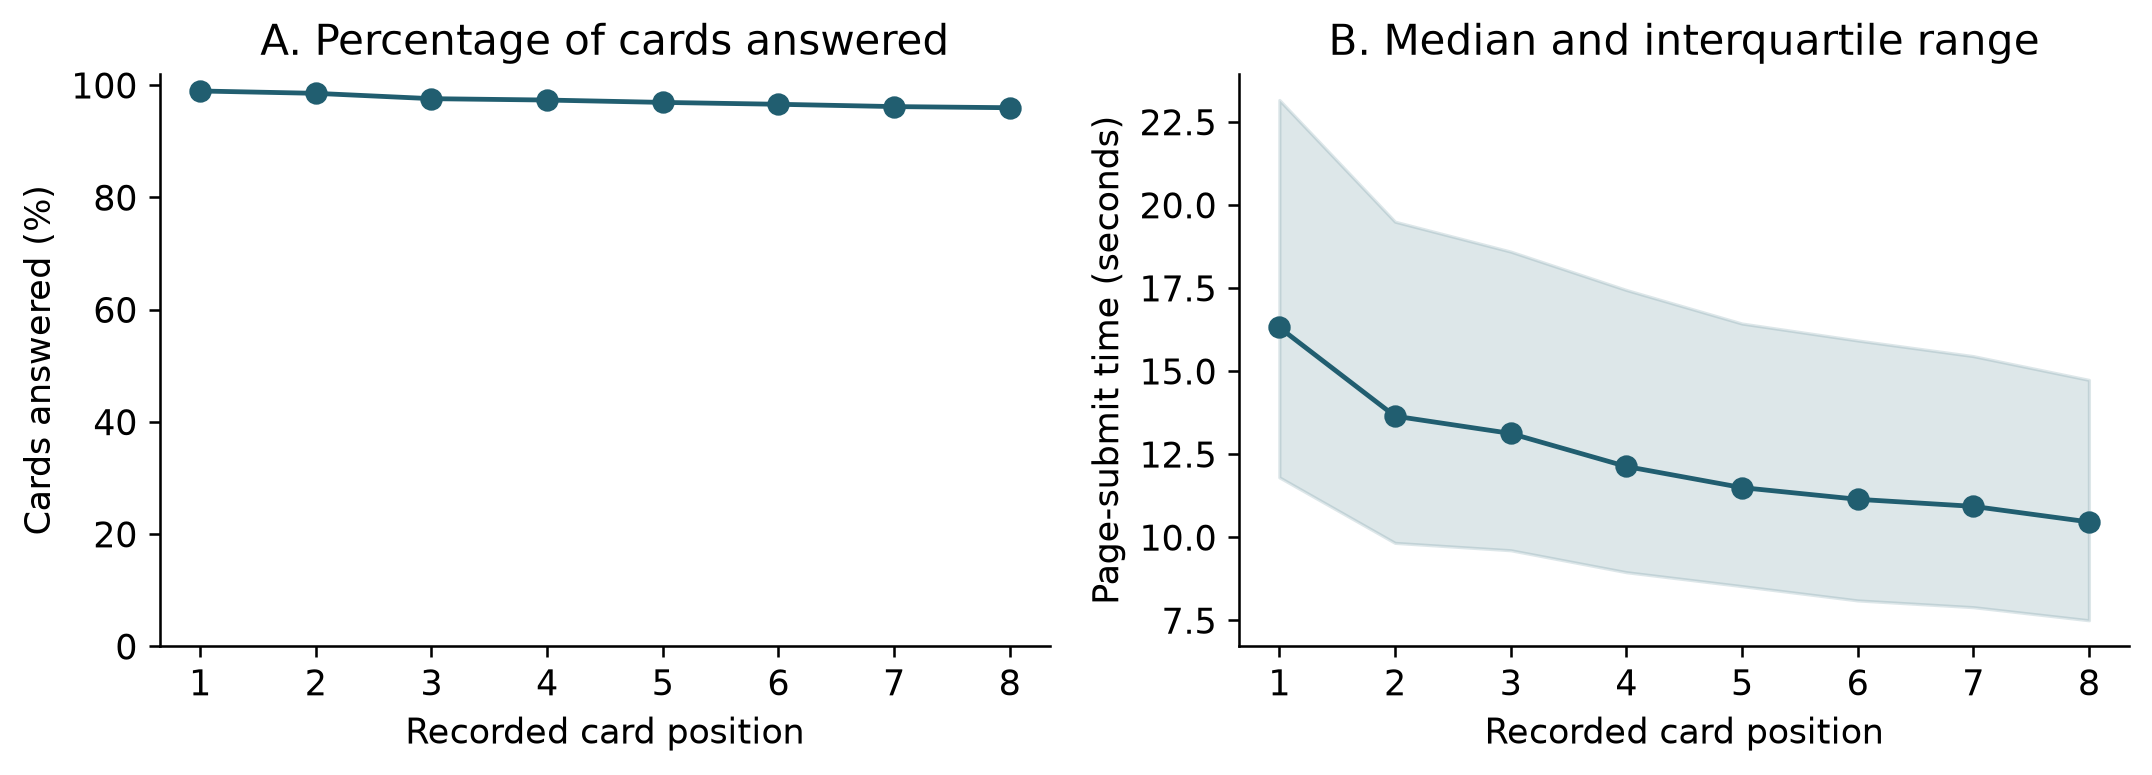
\includegraphics[width=.90\linewidth]{comparison_baseline/task_progression.png}}
\caption*{\textcolor{deletedreview}{\textbf{Deleted / superseded --- baseline Figure 5.} Recorded progression through the card task. Panel A shows the percentage of cards answered among eligible ordered entries. Panel B shows the median and interquartile range of positive page-submit times. Example-ambiguous identifiers are omitted from both panels.}}
\endgroup\end{figure}


\DIFdelend \DIFaddbegin 
\begin{figure}[!htbp]
\centering\begingroup\color{addedreview}
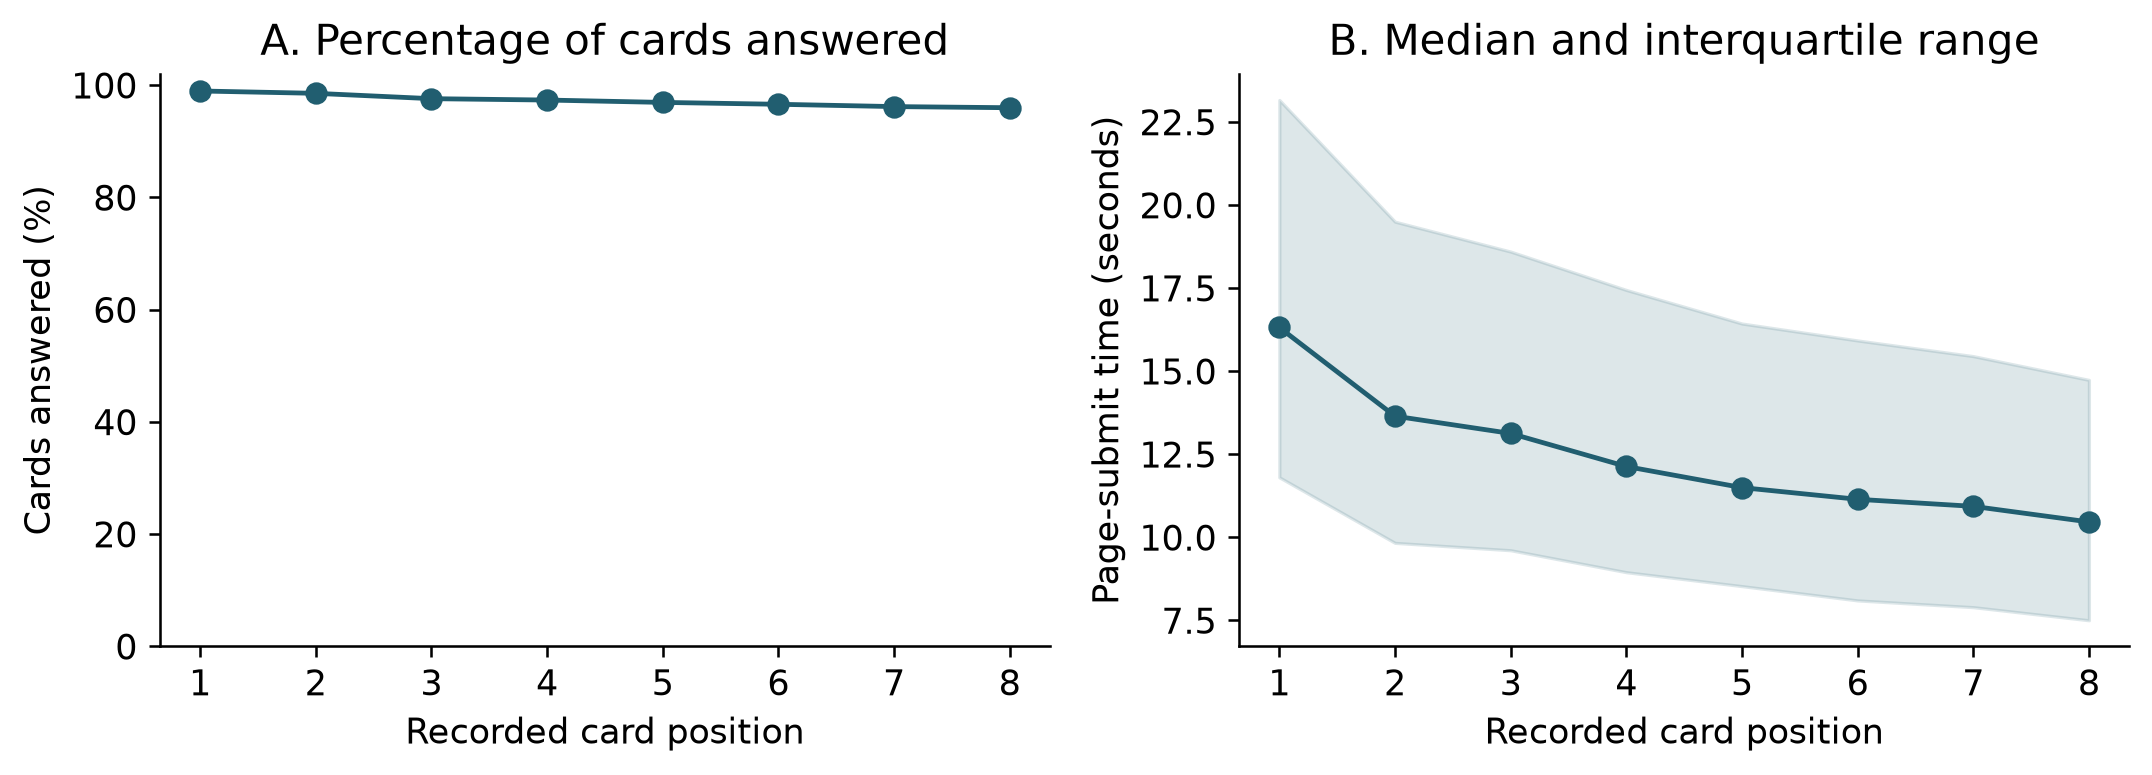
\includegraphics[width=.94\linewidth]{../../3. Output/paper_A/figures/task_progression.png}
\caption{\textcolor{addedreview}{Recorded progression through nonshared experimental positions in screened-in sequences. Panel A shows the percentage of cards answered; panel B shows the median and interquartile range of positive page-submit times.}}\label{fig:progression}
\endgroup\end{figure}


\DIFaddend 



Faster responses can reflect familiarization, reduced deliberation or fatigue; the\DIFaddbegin \DIFadd{se}\DIFaddend  timing fields do not distinguish the\DIFdelbegin \DIFdel{se}\DIFdelend  explanations. They record page submission rather than uninterrupted active reading.

\DIFdelbegin \DIFdel{Existing checks on complete ordered sequences also provide no convincing evidence of compensatory switching: the observed switching rate is 47.45 percent, against 47.14 percent under within-teacher reordering ($p=0.397$). 

}\DIFdelend 

\subsection{Comparison with regional teacher composition}
Figure~\ref{fig:population} compares univariate distributions with \DIFdelbegin \DIFdel{the supplied }\DIFdelend regional teaching statistics for 2023/24. Relative to that population, the \DIFaddbegin \DIFadd{decision }\DIFaddend sample contains more public-school teachers (93.0 versus 86.1 percent) \DIFdelbegin \DIFdel{, more teachers aged 45--54 (42.1 versus 34.3 percent), }\DIFdelend and fewer women among classifiable responses (\DIFdelbegin \DIFdel{67.3 }\DIFdelend \DIFaddbegin \DIFadd{67.7 }\DIFaddend versus 70.8 percent). The \DIFdelbegin \DIFdel{largest provincial shortfall is 3.2 percentage points}\DIFdelend \DIFaddbegin \DIFadd{figure also displays age, province and educational stage}\DIFaddend ; provinces are anonymized\DIFdelbegin \DIFdel{in the figure}\DIFdelend . Complete cases closely resemble \DIFdelbegin \DIFdel{all teachers with decisions }\DIFdelend \DIFaddbegin \DIFadd{the full decision sample }\DIFaddend on these margins.


\DIFdelbegin 
\begin{figure}[!htbp]
\centering\begingroup\color{deletedreview}
\setlength{\fboxsep}{3pt}\fcolorbox{deletedreview}{white}{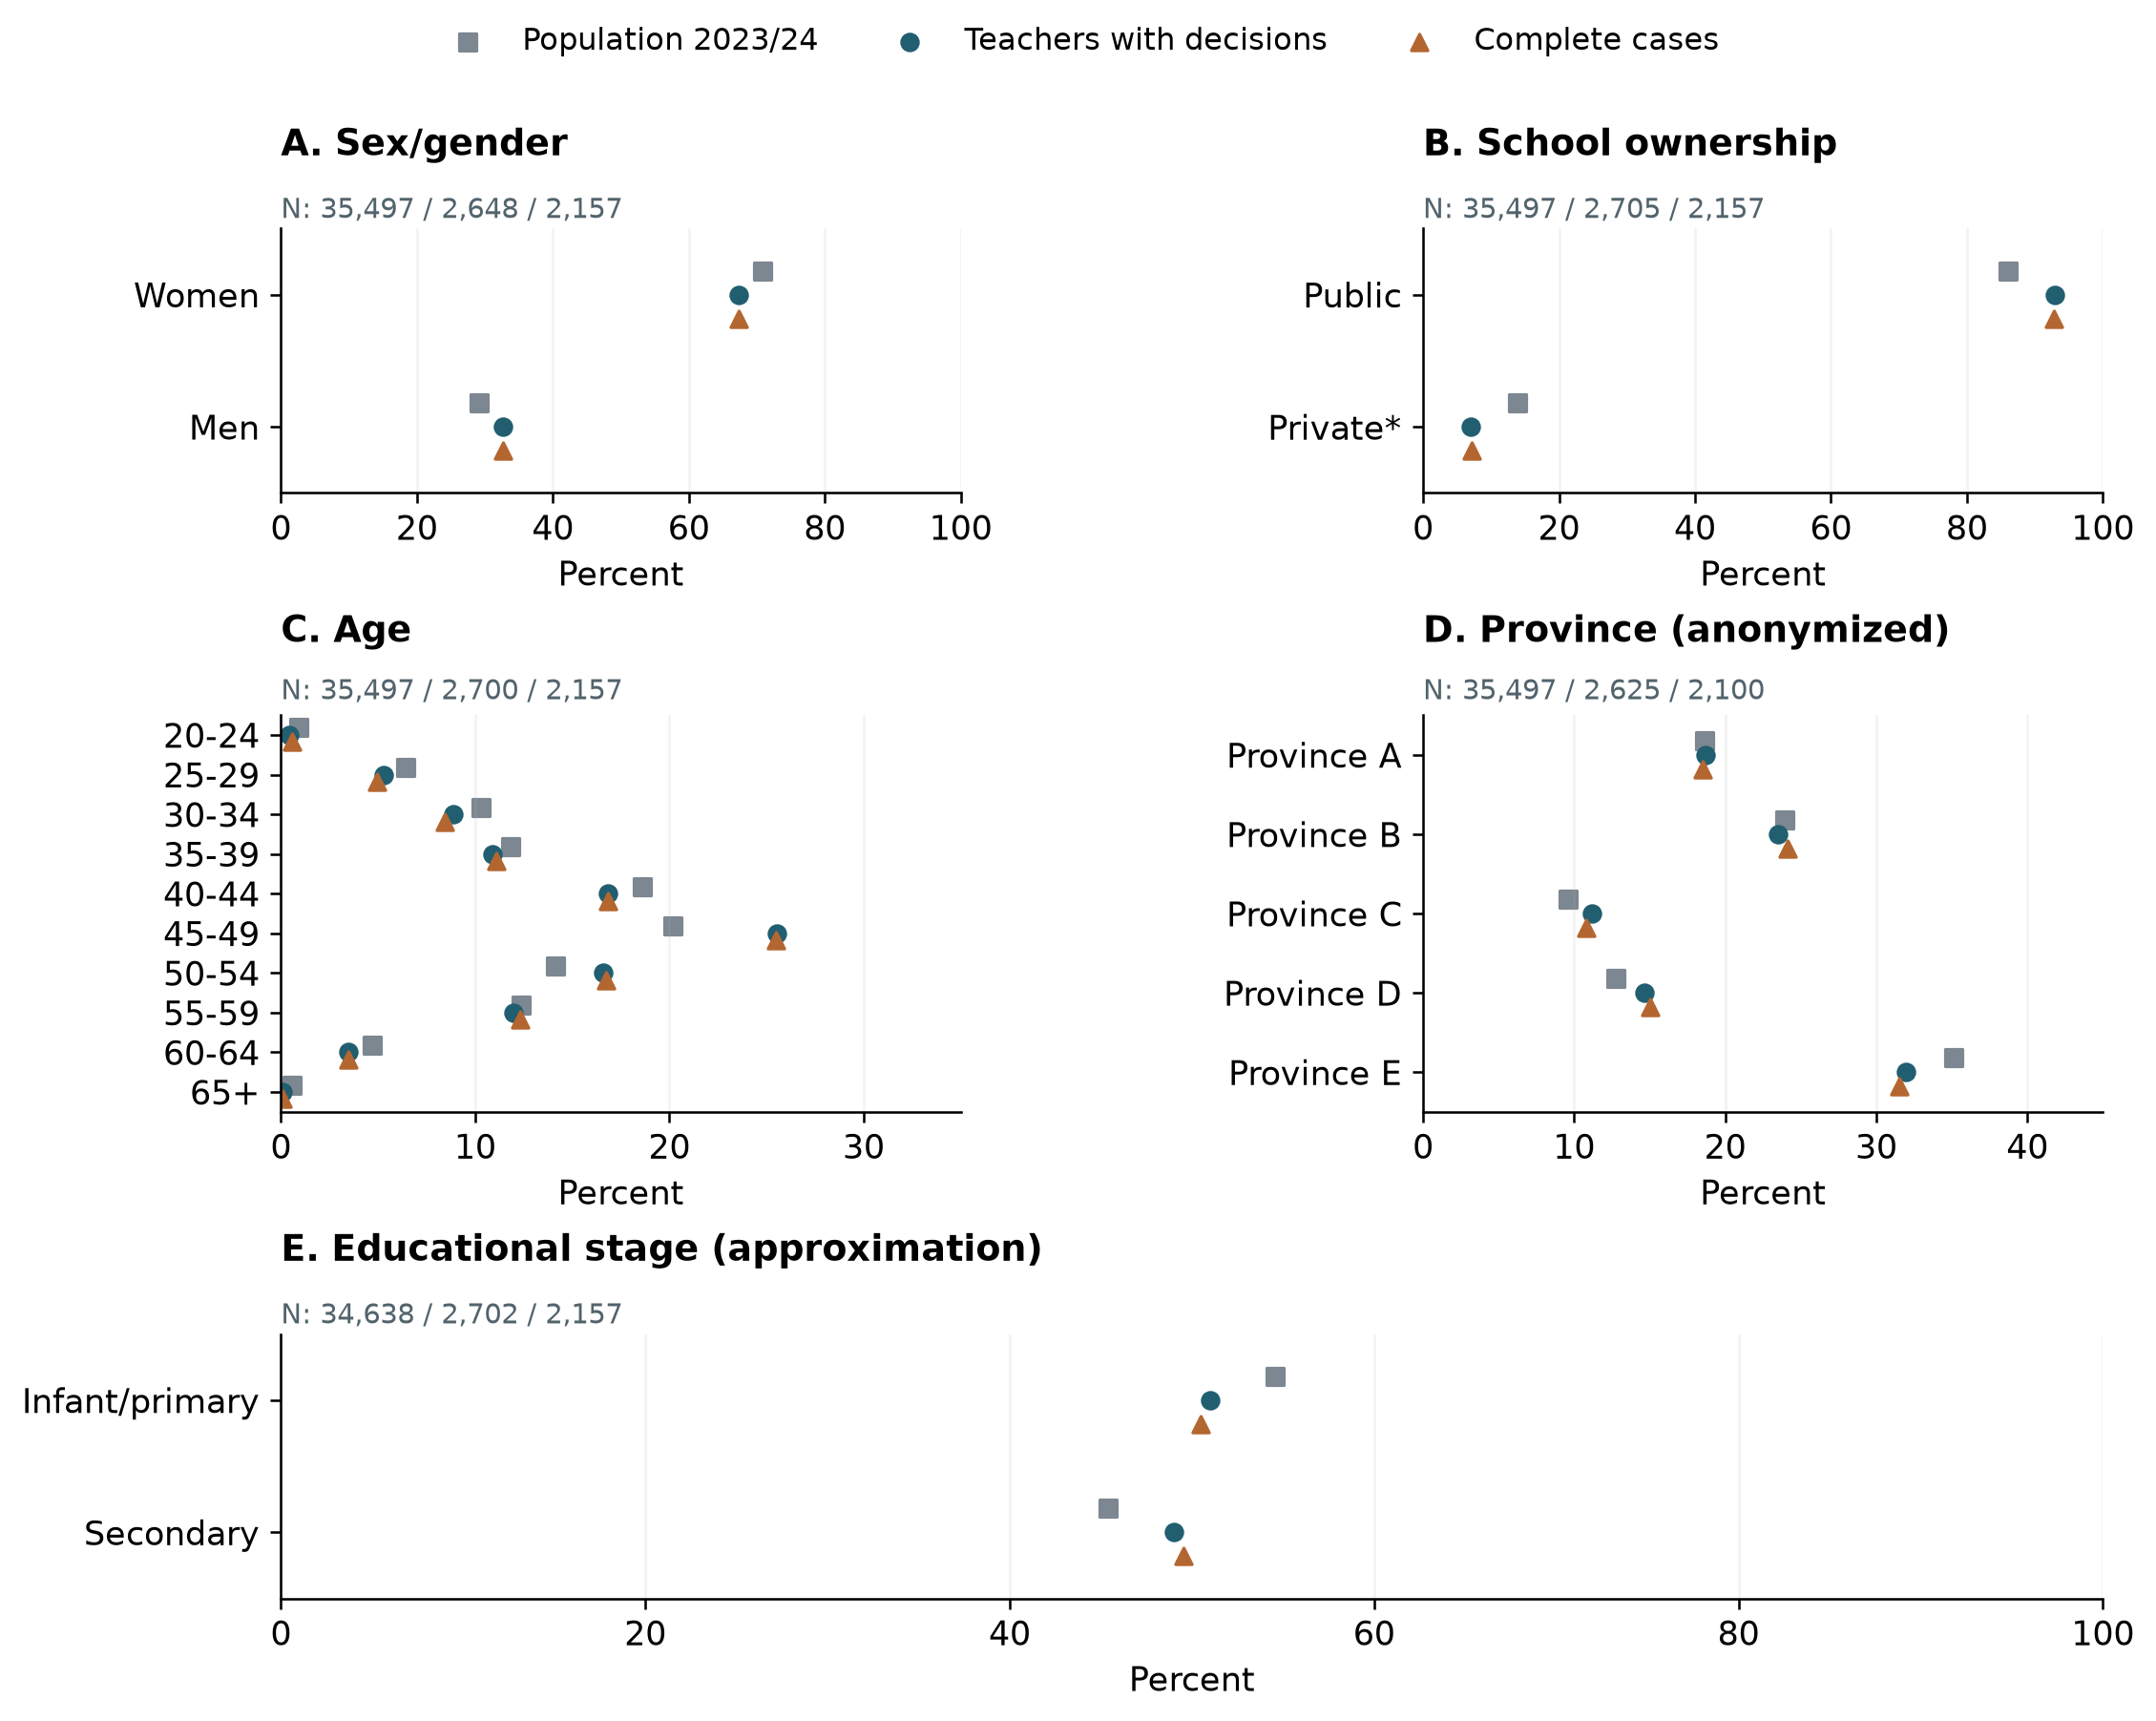
\includegraphics[width=.90\linewidth]{comparison_baseline/population_grid.png}}
\caption*{\textcolor{deletedreview}{\textbf{Deleted / superseded --- baseline Figure 6.} Univariate distributions in the regional population, the decision sample and the revised complete-case sample. Denominators follow the legend order. Percentages use classifiable observations; horizontal scales vary by panel. Private includes publicly funded private schools.}}
\endgroup\end{figure}


\DIFdelend \DIFaddbegin 
\begin{figure}[!htbp]
\centering\begingroup\color{addedreview}
\includegraphics[width=.94\linewidth]{../../3. Output/paper_A/figures/population_grid.png}
\caption{\textcolor{addedreview}{Univariate distributions in the regional population, the decision sample and the complete-case sample. Denominators follow the legend order. Percentages use classifiable observations; scales vary by panel. Private includes publicly funded private schools.}}\label{fig:population}
\endgroup\end{figure}


\DIFaddend 



The reference \DIFdelbegin \DIFdel{is the last available administrative statistics workbook for }\DIFdelend \DIFaddbegin \DIFadd{workbook covers }\DIFaddend 2023/\DIFdelbegin \DIFdel{24. The survey was conducted in spring 2025. }\DIFdelend \DIFaddbegin \DIFadd{24, preceding the spring 2025 survey. }\DIFaddend Province is derived from the declared school postal code, without IP-based imputation\DIFdelbegin \DIFdel{; 80 sample records are not classifiable. Gender has 57 unclassified responses , age five missing values, and stage three. The }\DIFdelend \DIFaddbegin \DIFadd{. Panel denominators exclude unclassified responses and are printed in the figure. The approximate }\DIFaddend stage comparison groups infant/primary and secondary teaching\DIFdelbegin \DIFdel{approximately}\DIFdelend , excluding 855 reference records in mixed, special and other categories. \DIFdelbegin \DIFdel{It uses 34,638 teachers; that }\DIFdelend \DIFaddbegin \DIFadd{Its }\DIFaddend source sheet totals 35,493 \DIFdelbegin \DIFdel{, versus }\DIFdelend \DIFaddbegin \DIFadd{teachers, compared with }\DIFaddend 35,497 in the other sheets. These \DIFdelbegin \DIFdel{differences of coverage }\DIFdelend \DIFaddbegin \DIFadd{coverage differences }\DIFaddend are retained explicitly. The \DIFdelbegin \DIFdel{figure }\DIFdelend \DIFaddbegin \DIFadd{comparison }\DIFaddend describes composition rather than establishing representativeness in unobserved beliefs or decisions.


\section{\DIFdelbegin \DIFdel{Alternative }\DIFdelend \DIFaddbegin \DIFadd{Supporting estimates and alternative }\DIFaddend definitions of harshness}\label{app:harshness}
\DIFaddbegin \DIFadd{Tables~\ref{tab:attr}--\ref{tab:academic} provide the numerical estimates underlying the main coefficient and academic-profile figures and the interaction discussion. Significance stars and standard errors follow the conventions defined in the main text.

}



\begin{table}[!htbp]
\centering\begingroup\color{addedreview}
\caption{\textcolor{addedreview}{Within-teacher responses to student attributes}}\label{tab:attr}
\small
\begin{tabular}{lr}
\toprule
Attribute & Coefficient (SE) \\
\midrule
Three or more failed subjects & \shortstack{54.70$^{***}$\\{\scriptsize (0.71)}} \\
Low basic competences & \shortstack{27.11$^{***}$\\{\scriptsize (0.63)}} \\
Frequent unjustified absence & \shortstack{6.72$^{***}$\\{\scriptsize (0.43)}} \\
Serious disciplinary problems & \shortstack{4.78$^{***}$\\{\scriptsize (0.47)}} \\
Male student & \shortstack{0.40\\{\scriptsize (0.47)}} \\
Complex social background & \shortstack{-1.76$^{***}$\\{\scriptsize (0.45)}} \\
\bottomrule
\end{tabular}
\tabnote{Coefficients in percentage points from additive teacher fixed-effect models; teacher-clustered SE. 20,452 decisions from 2,589 teachers. $^{*}p<.05$, $^{**}p<.01$, $^{***}p<.001$. SE in parentheses.}

\endgroup\end{table}








\begin{table}[!htbp]
\centering\begingroup\color{addedreview}
\caption{\textcolor{addedreview}{Combining academic and behavioral information within teachers}}\label{tab:interactions}
\small
\begin{tabular}{lr}
\toprule
Term & Coefficient (SE) \\
\midrule
Male student & \shortstack{0.38\\{\scriptsize (0.47)}} \\
Complex social background & \shortstack{-1.75$^{***}$\\{\scriptsize (0.45)}} \\
Three or more failed subjects & \shortstack{47.89$^{***}$\\{\scriptsize (1.10)}} \\
Low basic competences & \shortstack{21.45$^{***}$\\{\scriptsize (0.78)}} \\
Frequent unjustified absence & \shortstack{5.67$^{***}$\\{\scriptsize (0.54)}} \\
Serious disciplinary problems & \shortstack{2.75$^{***}$\\{\scriptsize (0.62)}} \\
Failures $\times$ low competences & \shortstack{11.07$^{***}$\\{\scriptsize (1.21)}} \\
Failures $\times$ absence & \shortstack{1.26\\{\scriptsize (0.93)}} \\
Failures $\times$ discipline & \shortstack{2.18$^{*}$\\{\scriptsize (0.92)}} \\
\bottomrule
\end{tabular}
\tabnote{Teacher fixed effects, 20,452 decisions, 2,589 teachers. Teacher-clustered SE. Stars for the three interactions use Holm-adjusted p-values. All coefficients are percentage points. $^{*}p<.05$, $^{**}p<.01$, $^{***}p<.001$. SE in parentheses.}

\endgroup\end{table}








\begin{table}[!htbp]
\centering\begingroup\color{addedreview}
\caption{\textcolor{addedreview}{Academic profiles and disagreement on the same six-attribute profile}}\label{tab:academic}
\small
\begin{tabular}{p{5.5cm}rrr}
\toprule
Failed subjects / competences & Repeat (\%) & SE & Disagree (\%) \\
\midrule
Fewer than three / adequate competence & 2.92 & 0.24 & 5.60 \\
Fewer than three / low competence & 23.79 & 0.77 & 35.60 \\
Three or more / adequate competence & 51.52 & 0.96 & 49.12 \\
Three or more / low competence & 85.76 & 0.60 & 24.33 \\
\bottomrule
\end{tabular}
\tabnote{Observed category rates with teacher-clustered SE. Disagreement compares two distinct teachers evaluating the same six-attribute profile and averages those probabilities by profile frequency within category. Other attributes are not standardized. No zero-mean hypothesis tests are attached to descriptive rates.}

\endgroup\end{table}





\FloatBarrier

\DIFaddend Table~\ref{tab:alternatives} compares four definitions using the revised covariates on identical complete cases. $H^a$ is the raw teacher repetition mean. $H^b$ is the preferred \DIFdelbegin \DIFdel{same-card }\DIFdelend \DIFaddbegin \DIFadd{same-profile }\DIFaddend relative measure. $H^c$ averages residuals from a pooled logistic model of the six attributes; $H^d$ additionally adjusts that model for stage and the three original ownership categories. Age and resource agreement retain similar coefficients. The secondary-stage association is \DIFdelbegin \DIFdel{3.33 }\DIFdelend \DIFaddbegin \DIFadd{3.43 }\DIFaddend points for $H^b$ but only \DIFdelbegin \DIFdel{0.17 }\DIFdelend \DIFaddbegin \DIFadd{0.18 }\DIFaddend points for $H^d$, which already removes stage-related variation in constructing the outcome. That change reflects the definition, not evidence that stage never mattered.


\DIFdelbegin 
\begin{table}[!htbp]
\centering\begingroup\color{deletedreview}
\caption*{\textcolor{deletedreview}{\textbf{Deleted / superseded --- baseline Table 7.} Characterization under four definitions of harshness}}
\small
\begin{tabular}{p{5.6cm}rrrr}
\toprule
Characteristic & $H^a$ & $H^b$ & $H^c$ & $H^d$ \\
\midrule
Constant & \shortstack{49.01$^{***}$\\{\scriptsize (4.77)}} & \shortstack{4.27\\{\scriptsize (4.70)}} & \shortstack{4.19\\{\scriptsize (4.68)}} & \shortstack{5.72\\{\scriptsize (4.68)}} \\
Secondary stage & \shortstack{3.47$^{***}$\\{\scriptsize (0.94)}} & \shortstack{3.33$^{***}$\\{\scriptsize (0.91)}} & \shortstack{3.27$^{***}$\\{\scriptsize (0.91)}} & \shortstack{0.17\\{\scriptsize (0.91)}} \\
Experience (years) & \shortstack{0.02\\{\scriptsize (0.08)}} & \shortstack{0.03\\{\scriptsize (0.08)}} & \shortstack{0.03\\{\scriptsize (0.08)}} & \shortstack{0.02\\{\scriptsize (0.08)}} \\
Female teacher & \shortstack{-0.08\\{\scriptsize (0.89)}} & \shortstack{-0.38\\{\scriptsize (0.87)}} & \shortstack{-0.40\\{\scriptsize (0.86)}} & \shortstack{-0.38\\{\scriptsize (0.86)}} \\
Age (years) & \shortstack{-0.28$^{***}$\\{\scriptsize (0.08)}} & \shortstack{-0.30$^{***}$\\{\scriptsize (0.08)}} & \shortstack{-0.29$^{***}$\\{\scriptsize (0.08)}} & \shortstack{-0.29$^{***}$\\{\scriptsize (0.08)}} \\
Public school & \shortstack{-0.22\\{\scriptsize (1.58)}} & \shortstack{-0.07\\{\scriptsize (1.50)}} & \shortstack{-0.09\\{\scriptsize (1.49)}} & \shortstack{-0.10\\{\scriptsize (1.48)}} \\
Reported permanent public appointment & \shortstack{-0.09\\{\scriptsize (1.15)}} & \shortstack{0.03\\{\scriptsize (1.10)}} & \shortstack{0.08\\{\scriptsize (1.09)}} & \shortstack{0.08\\{\scriptsize (1.09)}} \\
Teaching groups & \shortstack{0.08\\{\scriptsize (0.15)}} & \shortstack{0.05\\{\scriptsize (0.14)}} & \shortstack{0.06\\{\scriptsize (0.14)}} & \shortstack{0.06\\{\scriptsize (0.14)}} \\
Perceived teacher impact (0--10) & \shortstack{0.28\\{\scriptsize (0.28)}} & \shortstack{0.13\\{\scriptsize (0.28)}} & \shortstack{0.11\\{\scriptsize (0.28)}} & \shortstack{0.10\\{\scriptsize (0.28)}} \\
Empathy (1--5) & \shortstack{0.00\\{\scriptsize (0.70)}} & \shortstack{0.05\\{\scriptsize (0.70)}} & \shortstack{0.08\\{\scriptsize (0.70)}} & \shortstack{0.07\\{\scriptsize (0.69)}} \\
Effort attribution (1--10) & \shortstack{0.46$^{*}$\\{\scriptsize (0.23)}} & \shortstack{0.40\\{\scriptsize (0.23)}} & \shortstack{0.40\\{\scriptsize (0.23)}} & \shortstack{0.40\\{\scriptsize (0.23)}} \\
Excess resources for repeaters (0--10) & \shortstack{0.90$^{***}$\\{\scriptsize (0.15)}} & \shortstack{0.88$^{***}$\\{\scriptsize (0.15)}} & \shortstack{0.89$^{***}$\\{\scriptsize (0.15)}} & \shortstack{0.89$^{***}$\\{\scriptsize (0.15)}} \\
Teachers & 2157 & 2157 & 2157 & 2157 \\
$R^2$ (\%) & 4.63 & 4.82 & 4.85 & 3.98 \\
\bottomrule
\end{tabular}
\tabnote{Identical 2,157 complete cases and $X_3$ covariates. Coefficients in percentage points, HC3 SE. $H^a$: raw mean; $H^b$: same-card reference; $H^c$: attribute-logit residual; $H^d$: residual additionally adjusted for stage and ownership. $^{*}p<.05$, $^{**}p<.01$, $^{***}p<.001$. SE in parentheses. HC3 stars use the asymptotic normal reference.}

\endgroup\end{table}


\DIFdelend \DIFaddbegin 
\begin{table}[!htbp]
\centering\begingroup\color{addedreview}
\caption{\textcolor{addedreview}{Characterization under four definitions of harshness}}\label{tab:alternatives}
\small
\begin{tabular}{p{5.6cm}rrrr}
\toprule
Characteristic & $H^a$ & $H^b$ & $H^c$ & $H^d$ \\
\midrule
Constant & \shortstack{43.68$^{***}$\\{\scriptsize (4.77)}} & \shortstack{5.21\\{\scriptsize (4.66)}} & \shortstack{4.96\\{\scriptsize (4.64)}} & \shortstack{6.65\\{\scriptsize (4.64)}} \\
Secondary stage & \shortstack{3.60$^{***}$\\{\scriptsize (0.95)}} & \shortstack{3.43$^{***}$\\{\scriptsize (0.90)}} & \shortstack{3.37$^{***}$\\{\scriptsize (0.90)}} & \shortstack{0.18\\{\scriptsize (0.90)}} \\
Experience (years) & \shortstack{-0.01\\{\scriptsize (0.08)}} & \shortstack{0.01\\{\scriptsize (0.08)}} & \shortstack{0.01\\{\scriptsize (0.08)}} & \shortstack{0.00\\{\scriptsize (0.08)}} \\
Female teacher & \shortstack{0.03\\{\scriptsize (0.90)}} & \shortstack{-0.07\\{\scriptsize (0.86)}} & \shortstack{-0.08\\{\scriptsize (0.86)}} & \shortstack{-0.05\\{\scriptsize (0.86)}} \\
Age (years) & \shortstack{-0.24$^{**}$\\{\scriptsize (0.08)}} & \shortstack{-0.27$^{***}$\\{\scriptsize (0.08)}} & \shortstack{-0.27$^{***}$\\{\scriptsize (0.08)}} & \shortstack{-0.27$^{***}$\\{\scriptsize (0.08)}} \\
Public school & \shortstack{-0.28\\{\scriptsize (1.60)}} & \shortstack{-0.39\\{\scriptsize (1.49)}} & \shortstack{-0.39\\{\scriptsize (1.49)}} & \shortstack{-0.53\\{\scriptsize (1.48)}} \\
Reported permanent public appointment & \shortstack{0.09\\{\scriptsize (1.17)}} & \shortstack{0.41\\{\scriptsize (1.11)}} & \shortstack{0.43\\{\scriptsize (1.11)}} & \shortstack{0.43\\{\scriptsize (1.11)}} \\
Teaching groups & \shortstack{0.05\\{\scriptsize (0.15)}} & \shortstack{0.01\\{\scriptsize (0.14)}} & \shortstack{0.02\\{\scriptsize (0.14)}} & \shortstack{0.02\\{\scriptsize (0.14)}} \\
Perceived teacher impact (0--10) & \shortstack{0.13\\{\scriptsize (0.28)}} & \shortstack{-0.03\\{\scriptsize (0.27)}} & \shortstack{-0.05\\{\scriptsize (0.27)}} & \shortstack{-0.05\\{\scriptsize (0.27)}} \\
Empathy (1--5) & \shortstack{-0.18\\{\scriptsize (0.71)}} & \shortstack{-0.08\\{\scriptsize (0.70)}} & \shortstack{-0.06\\{\scriptsize (0.70)}} & \shortstack{-0.06\\{\scriptsize (0.70)}} \\
Effort attribution (1--10) & \shortstack{0.52$^{*}$\\{\scriptsize (0.23)}} & \shortstack{0.39\\{\scriptsize (0.22)}} & \shortstack{0.40\\{\scriptsize (0.22)}} & \shortstack{0.40\\{\scriptsize (0.22)}} \\
Excess resources for repeaters (0--10) & \shortstack{0.91$^{***}$\\{\scriptsize (0.15)}} & \shortstack{0.88$^{***}$\\{\scriptsize (0.15)}} & \shortstack{0.89$^{***}$\\{\scriptsize (0.15)}} & \shortstack{0.89$^{***}$\\{\scriptsize (0.15)}} \\
Teachers & 2164 & 2164 & 2164 & 2164 \\
$R^2$ (\%) & 4.49 & 4.68 & 4.73 & 3.77 \\
\bottomrule
\end{tabular}
\tabnote{Identical 2,164 complete cases and $X_3$ covariates. Coefficients in percentage points, HC3 SE. $H^a$: raw mean; $H^b$: same-profile reference; $H^c$: attribute-logit residual; $H^d$: residual additionally adjusted for stage and ownership. $^{*}p<.05$, $^{**}p<.01$, $^{***}p<.001$. SE in parentheses. HC3 stars use a t reference with residual degrees of freedom.}

\endgroup\end{table}


\DIFaddend 



\section{Decomposition: estimation and numerical diagnostics}\label{app:prediction}
The model and allocation are defined in the main text. The fixed design has full rank (34 columns)\DIFaddbegin \DIFadd{. The covariance design maps have full rank for the diagonal (6 variance parameters), three-pair (9) and unrestricted (21) specifications, including a distinct residual-variance direction. Both optimizers give virtually identical objectives and shares. The diagonal model has a positive-definite covariance}\DIFaddend , \DIFdelbegin \DIFdel{and the six random slopes have 21 unrestricted covariance parameters. }\DIFdelend \DIFaddbegin \DIFadd{a scaled-gradient diagnostic below 0.002 and a positive-definite Hessian. }\DIFaddend The \DIFdelbegin \DIFdel{fitted covarianceis nonsingular, the optimizer returns success and the Hessianis positive definite. The coefficient on observed harshness is approximately 0.968. These checks concern estimation of the specified model, not validation of the measure as a persistent teacher trait. }\DIFdelend \DIFaddbegin \DIFadd{richer covariance models fit better by REML AIC but have a near-zero covariance eigenvalue. We retain them as boundary sensitivities rather than interpreting all covariance directions as separately supported. Table~\ref{tab:covariance} discloses their fit and allocations; every component differs from the primary estimate by less than one percentage point.

}\DIFaddend 



\DIFaddbegin 
\begin{table}[!htbp]
\centering\begingroup\color{addedreview}
\caption{\textcolor{addedreview}{Covariance assumptions and model-implied variance allocation}}\label{tab:covariance}
\small
\begin{tabular}{p{4.7cm}rrr}
\toprule
Component & Diagonal & Three pairs & Unrestricted \\
\midrule
Student information & 47.93 & 48.64 & 48.53 \\
\shortstack[l]{Professional /\\demographic} & 0.18 & 0.17 & 0.18 \\
Beliefs & 0.18 & 0.18 & 0.18 \\
Observed harshness & 12.78 & 12.73 & 12.86 \\
Attribute sensitivities & 18.80 & 18.29 & 18.76 \\
Residual & 20.12 & 19.99 & 19.49 \\
Covariance parameters & 6 & 9 & 21 \\
Boundary estimate & No & Yes & Yes \\
REML AIC & 5787.63 & 5066.51 & 4990.23 \\
\bottomrule
\end{tabular}
\tabnote{Same 17,312 decisions and fixed design in all columns. Entries are percentages of model-implied variance. The diagonal specification is primary; the other specifications are boundary solutions. Two optimizers agree on the objective and allocations. AIC describes working-model fit, not validation of a generative model for response-derived harshness.}

\endgroup\end{table}






\DIFaddend For uncertainty, we resample the 2,\DIFdelbegin \DIFdel{705 }\DIFdelend \DIFaddbegin \DIFadd{604 }\DIFaddend teachers with usable decisions, retaining \DIFdelbegin \DIFdel{all their observed cards. Each sampled copy receives a separate cluster identifier. Same-card reference rates }\DIFdelend \DIFaddbegin \DIFadd{each sampled record's cards and assigning repeated copies separate cluster identifiers. Profile references }\DIFaddend and harshness are rebuilt \DIFdelbegin \DIFdel{from the }\DIFdelend \DIFaddbegin \DIFadd{using the full }\DIFaddend resampled decision population \DIFdelbegin \DIFdel{; the model is then fitted on the resampled teachers with complete covariates. Attribute centering and all }\DIFdelend \DIFaddbegin \DIFadd{before selecting complete covariate cases. Centering and the }\DIFaddend four-block projections are recalculated \DIFaddbegin \DIFadd{in each replicate}\DIFaddend . Standard errors are the standard deviations of the \DIFdelbegin \DIFdel{resulting shares over numerically accepted resamples. }\DIFdelend \DIFaddbegin \DIFadd{shares over 199 teacher resamples, with the diagonal covariance specification held fixed. Each fit uses automatic initialization, full gradient and Hessian checks, and a second optimizer if those checks fail. }\DIFaddend All 199 \DIFdelbegin \DIFdel{draws returned optimizer success and finite allocations; one }\DIFdelend \DIFaddbegin \DIFadd{resamples passed the numerical checks; 17 }\DIFaddend had a boundary \DIFdelbegin \DIFdel{covariance estimate and was retained. Each bootstrap fit starts from the full-sample covariance estimates and uses tight optimization tolerances. We record optimizer success and boundaryfits; the full gradient and Hessian checks above refer to the point estimate}\DIFdelend \DIFaddbegin \DIFadd{variance estimate and were retained. These standard errors are descriptive bootstrap dispersion, not calibrated confidence intervals for variance parameters at a boundary. The resampling measures uncertainty conditional on the chosen model and reconstruction, not uncertainty about the invariance assumption for shared example fields}\DIFaddend .

The linear model describes \DIFdelbegin \DIFdel{variation on the response scale; its }\DIFdelend \DIFaddbegin \DIFadd{response-scale variation; approximately 29.2 percent of }\DIFaddend conditional fitted values \DIFdelbegin \DIFdel{need not be valid probabilities. Approximately 25.5 percent lie }\DIFdelend \DIFaddbegin \DIFadd{fall }\DIFaddend outside $[0,1]$. \DIFdelbegin \DIFdel{We therefore interpret the allocation as }\DIFdelend \DIFaddbegin \DIFadd{Its allocation is therefore }\DIFaddend a working-model description\DIFdelbegin \DIFdel{and do not use it to assign }\DIFdelend \DIFaddbegin \DIFadd{, not a set of }\DIFaddend individual retention probabilities. The \DIFdelbegin \DIFdel{random-slope share includes cross-attribute covariance and is not further divided into six independent percentages}\DIFdelend \DIFaddbegin \DIFadd{coefficient on observed harshness is approximately 0.965. Because harshness is computed from the response itself, the total model-implied variance need not equal the empirical variance of the binary outcome; the six shares divide the denominator in Equation~\ref{eq:variance_total}. Richer covariance assumptions alter this accounting only modestly, but they do not validate it as a causal or psychological decomposition}\DIFaddend .
\end{document}
